% based on IEEE template, adapted by Tim Bruedigam and students

\documentclass[conference]{IEEEtran}
\IEEEoverridecommandlockouts

%\usepackage{cite}
\usepackage{amsmath,amssymb,amsfonts}
\usepackage{algorithmic}
\usepackage{graphicx}
\usepackage{textcomp}
%\usepackage[utf8]{inputenc}
\usepackage[]{todonotes}
\usepackage{hyperref}
\newcommand{\chapter}{\section}
%\def\BibTeX{{\rm B\kern-.05em{\sc i\kern-.025em b}\kern-.08em
%    T\kern-.1667em\lower.7ex\hbox{E}\kern-.125emX}}

%%%%%%%%%%%%%%%%%%%%%%%%%%%%%%%%%%%%%%%%%%%%%%%%%%%%%%%%%%%%%%
% CUSTOMIZING Tex-File for students to be adjusted as needed %
%%%%%%%%%%%%%%%%%%%%%%%%%%%%%%%%%%%%%%%%%%%%%%%%%%%%%%%%%%%%%%
%%%%%%%%%%%%%%%%%%%%%
% CUSTOM PACKAGES	%
%%%%%%%%%%%%%%%%%%%%%
\usepackage{tikz}
\usepackage{pgfplots}
\usepackage{textgreek}
\usepackage{dsfont}
\usepackage{caption}
\usepackage{subcaption}
\usepackage{flushend}

% \usepackage{IEEEtrantools}

%%%%%%%%%%%%%%%%%%%%%
% CUSTOM COMMANDS	%
%%%%%%%%%%%%%%%%%%%%%
% e.g. Math conventions as vectors, Matrices, sets
\renewcommand{\vec}[1]{\mathbf{\MakeLowercase{#1}}}
\newcommand{\Mat}[1]{\mathbf{\MakeUppercase{#1}}}
\newcommand{\set}[1]{\boldsymbol{#1}}

\makeatletter
\newcounter{manualsubequation}
\renewcommand{\themanualsubequation}{\alph{manualsubequation}}
\newcommand{\startsubequation}{%
  \setcounter{manualsubequation}{0}%
  \refstepcounter{equation}\ltx@label{manualsubeq\theequation}%
  \xdef\labelfor@subeq{manualsubeq\theequation}%
}
\newcommand{\tagsubequation}{%
  \stepcounter{manualsubequation}%
  \tag{\ref{\labelfor@subeq}\themanualsubequation}%
}
\let\subequationlabel\ltx@label
\makeatother

\DeclareMathOperator*{\argmin}{arg\,min}
\DeclareMathSymbol{\shortminus}{\mathbin}{AMSa}{"39}

% e.g. use differenc layers in tikz
\pgfdeclarelayer{background}
\pgfdeclarelayer{nodelayer}
\pgfdeclarelayer{edgelayer}
\pgfdeclarelayer{foreground}
\pgfsetlayers{background,edgelayer,nodelayer,main,foreground}
%%%%%%%%%%%%%%%%%%%%%
% HYPHENATIONS 		%
%%%%%%%%%%%%%%%%%%%%%
\hyphenation{Lya-pu-nov}

% %%%%%%%%%%%%%%%%%%%%%%%%%%%%%%%%%%%%%%%%%%%%%%%%%%%%%%%%%%%%%%
% NOTE: Using this is optional
% 	Nonetheless, feel free to include this file and adjust the 
% 	examples below as needed
%   
% Questions, feedback and improvements:
%	-> https://git.lsr.ei.tum.de/students/student-templates/issues
% ATTENTION:
% 	- Keep in mind that thif file uses the \vec and \mat commands
% 	 	which are defined in customize.tex!
%	- add glsaddall if you want all of the elements in gloss.aux
%		being printed into your list of acronyms.
% Further reading:
%	https://ctan.org/pkg/glossaries?lang=en
%%%%%%%%%%%%%%%%%%%%%%%%%%%%%%%%%%%%%%%%%%%%%%%%%%%%%%%%%%%%%%

% include packages
\usepackage{setspace}
\usepackage{filecontents}
% for sharelatex, the indexing using xindy:
% 	http://xindy.sourceforge.net/doc/faq-1.html#ss1.2
% is not available, thus the adjustments below ar necessary
%% Adjust Flag for Sharelatex
\newif\ifShareLatex 
%\ShareLatextrue            	% if you work in sharelatex: https://sharelatex.tum.de
\ShareLatexfalse          		% if you work locally

\ifShareLatex
    \usepackage[acronym, style=alttree, shortcuts, toc=true, nomain, nonumberlist]{glossaries}
    \renewcommand{\makeglossaries}{\makenoidxglossaries}
    \renewcommand{\printglossary}{\printnoidxglossary}
\else
    \usepackage[acronym,style=alttree, toc=true, shortcuts, xindy, nomain, nonumberlist]{glossaries}
    \RequirePackage[xindy]{imakeidx}
\fi

%%%%%%%%%%%%%%%%%%%%%%%%%%%%%%%%%%
% DEFINE HEADINGS AND CATEGORIES %
%%%%%%%%%%%%%%%%%%%%%%%%%%%%%%%%%%
% preferable use a command, to adjust the Capitalization 
% for the header section of fancyhdr automatically
\newcommand{\Symbols}{List of Symbols}
\newcommand{\Notation}{Notation}
\newglossary{symbols}{sym}{sbl}{\Symbols}
\newglossary{notation}{not}{nt}{\Notation}
% set width of first row
\glssetwidest{THISWIDE}     % adjust length as needed

%%%%%%%%%%%%%%%%%%%%%%%%%%%%%
% DEFINE ACRONYMS/GLOSSARY	%
%%%%%%%%%%%%%%%%%%%%%%%%%%%%%
\makeglossaries % don't remove this
\begin{filecontents}{gloss.aux}
	%===========%
	% ACRONYMS	%
	%===========%
	\newacronym{MPC}{MPC}{model-predictive control}
	\newacronym{BIBO}{BIBO}{bounded-input bounded-output}
	\newacronym{HRC}{HRC}{Human-Robot Collaboration}
	%============%
	% SYMBOLS	%
	%===========%
	\newglossaryentry{control}{type=symbols,
		sort={control},
		name={\ensuremath{\vec{u}}},
		description={control input vector}
	}
    \newglossaryentry{uk}{type=symbols,
		sort={control},
		name={\ensuremath{\vec{u}_k}},
		description={control input vector with time step}
	}
    \newglossaryentry{xk}{type=symbols,
		sort={state},
		name={\ensuremath{\vec{x}_k}},
		description={state vector with time step}
	}
	%============%
	% NOTATION	%
	%===========%
	\newglossaryentry{vector}{type=notation,
		sort={vector},
		name={\ensuremath{\vec{x}_n}},
		description={$n$-dimensional vector named $x$}
	}	
	\newglossaryentry{matrix}{type=notation,
		sort={vector-matrix},
		name={\ensuremath{\Mat{x}_{m\times n}}},
		plural={matrices},
		user1={Mat},
		description={\ensuremath{m\times n} dimensional Matrix  named \ensuremath{X}}
	}	
\end{filecontents}
\loadglsentries{gloss.aux}

%%%% Add GLOSSARIES at end of thesis
\newcommand{\AddMyGloss}{
	\renewcommand{\glsglossarymark}[1]{}
   	\printglossary[type=acronym]
	\markboth{\MakeUppercase{acronyms}}{\MakeUppercase{acronyms}}
  	\ifdefined\Symbols
		\printglossary[type=symbols, nogroupskip]
		\markboth{\MakeUppercase{\Symbols}}{\MakeUppercase{\Symbols}}
	\fi
	\ifdefined\Notation
		\printglossary[type=notation, nogroupskip]
		\markboth{\MakeUppercase{\Notation}}{\MakeUppercase{\Notation}}
	\fi
}

		% add your glossary in this file 

\begin{document}



%%%%%%%%%%%%%%%%%%%%%%%%%%%%% Title / Student %%%%%%%%%%%%%%%%%%%%%%%%%%%%%%%%
\title{Modeling the Impact of Public Traffic on COVID-19 Spread Rates in Germany}

\author{\IEEEauthorblockN{Tobias Krug}
\IEEEauthorblockA{\textit{Department of Electrical and Computer Engineering, Chair of Automatic Control Engineering (LSR)} \\
\textit{Technical University of Munich}\\
Munich, Germany\\
tobias.krug@tum.de}
}

\maketitle


%%%%%%%%%%%%%%%%%%%%%%%%%%%%% Document %%%%%%%%%%%%%%%%%%%%%%%%%%%%%%%%
\begin{abstract}
This report builds on the idea of the networked SEIR model to recover pandemic spread parameters and apply the identified model for simulation/prediction of pandemic activity based on COVID-19 case data, public transport schedule information and estimated mobility behavior of a population. A data-driven methodology to the problems of transient network structure recovery and time-varying strength of adjacency estimation is presented. A case study on German data is implemented and the resulting models' performances are evaluated numerically and graphically.
\end{abstract}

\begin{IEEEkeywords}
Epidemic modeling, System identification, Networked control systems, Data engineering
\end{IEEEkeywords}

\section{Introduction}

\subsection{Problem Statement}
This report deals with the specific situation of COVID-19 spreading in Germany. It aims to contribute to the field of COVID-19 spread models. Hereby, it helps to tackle the current lack of concepts that consider the unique combination of extensive public transport infrastructure and regionally differing COVID-19 legislation as is faced in Germany.

The lack of such a model is in equal parts attributable to:
\begin{itemize}
	\item the data collection avoidance due to the population's mindset valuing data privacy (GDPR et al.) and
	\item the niche role of digital solutions to everyday activities like commuting, which would allow data collection in the first place.
\end{itemize}

Hence, acquisition of actual usage data of public transport networks is complex and revolves around the combination of different (proxy) data sources; namely public transport schedules, behavior data and models of passengers and data sets to account for legislation and pandemic parameters on various geographical scopes.

\subsection{Related Work}
Pandemics in general and the COVID-19 pandemic caused by the spread of the SARS-CoV-2 virus specifically are of concern for a number of different academic entities and fields. The works that are of specific relevance for this report can be clustered into six categories:

\begin{enumerate}
	\item varying approaches to model pandemics \cite{zinoAnalysisPredictionControl2021}
	\item varying extensions of SIR models \cite{liuNewSEAIRDPandemic2021}, \cite{ramosSimpleComplexEnough2021} and the analysis of the model's accuracy and its sensitivity \cite{khoshnawQuantitativeQualitativeAnalysis2020}
 	\item global Markov Model approach \cite{frihiToolboxSimulateMitigate2021}
	\item impact of quarantine/lockdown on the pandemic spread \cite{wellsOptimalCOVID19Quarantine2021}, \cite{memonAssessingRoleQuarantine2021} and other special groups at risk \cite{kouidereOptimalControlMathematical2021}
	\item concepts to control the pandemic \cite{pintonetoMathematicalModelCOVID192021}, \cite{aravindakshanPreparingFutureCOVID192020}, its economic impact \cite{caulkinsOptimalLockdownIntensity2021} and how the right to demonstrate might conflict with pandemic containment \cite{langeSpreadingDiseaseProtest2021}
	\item approaches to track and predict spread in real time with mobility data \cite{leungRealtimeTrackingPrediction2021} or online search terms \cite{lamposTrackingCOVID19Using2021}
\end{enumerate}

The approach in this report builds on the paper and MATLAB implementation of Vrabac et al. \cite{vrabacCapturingEffectsTransportation2020}. The following section presents the prerequisites to apply it to data from Germany alongside the measures taken to improve the performance of the networked SEIR model.

\subsection{Problem Setup}
The problem setup consists of

\begin{itemize}
	\item raw, unrelated data from various sources and
	\item a prototypic MATLAB implementation of the networked SEIR model from \cite{vrabacCapturingEffectsTransportation2020}.
\end{itemize}

Based on this, a data processing pipeline to fuse the different data sets and transform them into a simulation ready format is presented. Subsequently, the parameters of a networked SEIR model are identified and tested using both factual initial conditions and behavior data and counterfactual behavior data to determine the sensitivity of the pandemic spread to changes of the population's mobility behavior.

\section{Technical Approach}
In this section, I present the concept to use mobility data, behavior data and pandemic data to calibrate and test a networked SEIR model. The theoretical concept of the networked SEIR model is introduced in \autoref{ssec:networkedSEIRModel}, which is followed by implementation specifics in \autoref{ssec:implementation}.

\subsection{Networked SEIR model}\label{ssec:networkedSEIRModel}

The idea of a networked SEIR model builds on the widely employed concept of epidemic models, that divide populations into compartments, whose relations are described as a set of differential equations. The basic SIR model is extended to the SEIR as introduced by \cite{aronSeasonalityPerioddoublingBifurcations1984} to account for epidemic scenarios in which humans are not immediately infectious after contact but have a static incubation period in becoming so. Therefore it is applicable to analyze virus-induced epidemics like COVID-19. Additional to the standard SEIR model, two sets of spread rates $\beta$ are introduced in equations 2 and 3 of \cite{vrabacCapturingEffectsTransportation2020}. While $\beta_{I1}, \beta_{I2}, \beta_{I3}$ relate to the standard SEIR model spread from infectious to exposed compartments, the new set of spread rates $\beta_{E1}, \beta_{E2}, \beta_{E3}$ allow to model the spread from exposed compartments to other exposed compartments.

The networked SEIR model from \cite{vrabacCapturingEffectsTransportation2020} takes this idea even further, in that it aims to identify spread parameters for a population divided into many subpopulations, which itself are divided into the SEIR compartments. Each of these subpopulations is modeled to influence the compartments of geographically adjacent regions by parameter $A1$, their own compartments by means of community spreading with parameter $A2$ and due to the travel behavior of humans inscribed by $A3$. $A1$, $A2$ and $A3$ are all so-called adjacency matrices, which model the strength of relationship between network entities. Entities relate to political counties in this analysis.

\subsubsection{Identifying the networked SEIR model parameters}\label{ssec:identifyNetworkedSEIR}
The identification of the networked SEIR model can be expressed as an optimization problem, that results from discretization of the system of continuous partial differential equations. The following brief discussion is based on the paper and prototypic implementation in \cite{vrabacCapturingEffectsTransportation2020}.

The optimization problem revolves around finding spread parameters that describe the pandemic spread across  a number of counties \eqref{eq:1}, for a number of time steps \eqref{eq:2} by using pandemic data with the sample rate $h$, which equals 1 in most scenarios.

% subequations?
\begin{equation}
\begin{aligned}
	m &= N_{counties} = const.% \label{eq:1}
\\ 
	n &= N_{timesteps} = const.% \label{eq:2}
\\
	j &\in \{1, 2, ..., n-1\}
\end{aligned}
\end{equation}

For each of these counties and days of analysis, a difference equation for the compartments exposed, infectious and removed describes the rate of change. The difference equations are expressed in vector form to simply the optimization problem, hence the input data matrices $E_{(n\times m)}$, $I_{(n\times m)}$ and $R_{(n\times m)}$ are reshaped\footnote{Notation refers to the MATLAB implementation \url{https://www.mathworks.com/help/matlab/ref/reshape.html}} as vectors $e$, $i$ and $r$. As we intend to identify one set of spread parameters common to all regions under analysis, the input case data matrices are expected to be normalized using each region's number of residents.

\begin{align}
\startsubequation\tagsubequation\label{eq:4a}
	e &= reshape(E_{(n\times m)}^T, n*m, 1)
\\
\tagsubequation\label{eq:4b}
	i &= reshape(I_{(n\times m)}^T, n*m, 1)
\\
\tagsubequation\label{eq:4c}
	r &= reshape(R_{(n\times m)}^T, n*m, 1)
\\
\tagsubequation\label{eq:4d}
	\Delta_e &= e_{(n+1:end)} - e_{(1:(m-1)*n)}
\\
\tagsubequation\label{eq:4e}
	\Delta_i &= i_{(n+1:end)} - i_{(1:(m-1)*n)}
\\
\tagsubequation\label{eq:4f}
	\Delta_r &= r_{(n+1:end)} - r_{(1:(m-1)*n)}
\\
	\Delta &= [\Delta_e ; \Delta_i ; \Delta_r]
\end{align}

While the adjacency matrices $A1$ (models adjacent county spread) and $A2$ (models intra-county spread) are static by nature, $A3$ (models mobility-driven spread) introduces time-dependent strength of connectedness, e.g. number of vehicles moving--and hence changes with each iteration $j$. To further consider the time-dependent mobility behavior of the population and policy behavior of the government, the parameters $\psi_{1_j}$, $\psi_{2_j}$ and $\psi_{3_j}$ are introduced. Depending on the data set, these can be either scalar values representing similar behavior in all counties or diagonal matrices, wherein each element of the diagonal describes the mobility behavior and policy information of one region under analysis. Extending the works of Vrabac et al., this work determines the parameters $\psi$ in a data-driven approach in \autoref{ssec:implementation}.

\begin{align}
\startsubequation\tagsubequation\label{eq:6a}
    A1_{s_j} &= \psi_{1_j} A1
\\
\tagsubequation\label{eq:6b}
    A2_{s_j} &= \psi_{2_j} A2
\\
\tagsubequation\label{eq:6c}
    A3_{s_j} &= \psi_{3_j} A3_j
\end{align}

The daily levels of each compartment \eqref{eq:4a}, \eqref{eq:4b} and \eqref{eq:4c} are then used to determine the discretized, time-dependent version of the networked SEIR model as described by \eqref{eq:8}. The networked SEIR model is then parametrized using the parameter vector $[\beta_{E1}, \beta_{E2}, \beta_{E3}, \beta_{I1}, \beta_{I2}, \beta_{I3}, \sigma, \gamma]$. These parameters are identified based on the optimization problem stated as \eqref{eq:9}, which is the minimum square normed difference of the parametrized networked SEIR model compartments and the actual daily difference of compartments given by the input data.

\begin{align}
\startsubequation\tagsubequation\label{eq:7a}
	S_j &= \mathds{1} - diag(e_j + i_j + r_j)
\\
\tagsubequation\label{eq:7b}
	e_j &= e_{(n*(j-1)+1:n*j)}
\\
\tagsubequation\label{eq:7c}
	i_j &= i_{(n*(j-1)+1:n*j)}
\\
\tagsubequation\label{eq:7d}
	r_j &= r_{(n*(j-1)+1:n*j)}
\\
\tagsubequation\label{eq:7e}
\begin{split}
	\delta_{e_j} &= h [S_j A1_{s_j} e_j, S_j A2_{s_j} e_j, S_j A3_{s_j} e_j,
	\\
	&\quad S_j A1_{s_j} i_j, S_j A2_{s_j} i_j, S_j A3_{s_j} i_j, -e_j, 0]
\end{split}
\\
\tagsubequation\label{eq:7f}
	\delta_{i_j} &= h [0, 0, 0, 0, 0, 0, e_j, i_j]
\\
\tagsubequation\label{eq:7g}
	\delta_{r_j} &= h [0, 0, 0, 0, 0, 0, 0, i_j]
\\
	\delta &= [\delta_e; \delta_i; \delta_r] \label{eq:8}
\\
	\begin{split}
		&[\beta_{E1}^*, \beta_{E2}^*, \beta_{E3}^*, \beta_{I1}^*, \beta_{I2}^*, \beta_{I3}^*, \sigma^*, \gamma^*] =
		\\
		&\argmin_{\beta_{E1}, \beta_{E2}, \beta_{E3}, \beta_{I1}, \beta_{I2}, \beta_{I3}, \sigma, \gamma}
		\\
		&\{\lVert \delta [\beta_{E1}, \beta_{E2}, \beta_{E3}, \beta_{I1}, \beta_{I2}, \beta_{I3}, \sigma, \gamma]^T - \Delta\rVert\} \label{eq:9}
	\end{split}
\end{align}

To ensure plausible results, the optimization problem is constrained. Firstly, the spread parameters are required to be non-negative \eqref{eq:10a}. Secondly, the incubation rate $\sigma$ is upper-bounded by a static time delay introduced to estimate the exposed compartment \eqref{eq:10b}. This delay shifts the data of the infectious compartment data - as derived from government agency data - by $\Delta_{t_{preExposed}}$ days into the past. Thirdly, the cure rate $\gamma$ is upper-bounded \eqref{eq:10c}. Lastly, the combined spread rates described by the parameters $\beta$ and the adjacency matrices $A$ are upper-bounded by the inverse of the sample rate $h$ for each time step $j$ and region $k \in \{1, 2, ..., m\}$ \eqref{eq:10d}.

\begin{align}
\startsubequation\tagsubequation\label{eq:10a}
	\beta_{E1}, \beta_{E2}, \beta_{E3}, \beta_{I1}, \beta_{I2}, \beta_{I3}, \sigma, \gamma &>= 0
\\
\tagsubequation\label{eq:10b}
	\sigma &<= 1/\Delta_{t_{preExposed}}
\\
\tagsubequation\label{eq:10c}
	\gamma &<= 1
\\
\tagsubequation\label{eq:10d}
\begin{split}
	\vert A1_{s_{j_{(k, 1:m)}}} \vert (\beta_{E1} + \beta_{I1}) &+ \vert A2_{s_{j_{(k, 1:m)}}} \vert (\beta_{E2} + \beta_{I2})
	\\
	+ \vert A3_{s_{j_{(k, 1:m)}}} \vert (\beta_{E3} + \beta_{I3}) &<= 1/h
\end{split}
\end{align}

\subsubsection{Simulating the networked SEIR Model}

Based on the parametrized networked SEIR model, we can calculate the pandemic spread per compartment, region and day. The entry point for the simulation is the set of initial conditions $\{s_{t0}, i_{t0}, e_{t0}, r_{t0}\}$, which describe the initial pandemic levels of each region, and the parameter vector $[\beta_{E1}, \beta_{E2}, \beta_{E3}, \beta_{I1}, \beta_{I2}, \beta_{I3}, \sigma, \gamma]$. Using \eqref{eq:6a}, \eqref{eq:6b} and \eqref{eq:6c} an iterative problem to determine the pandemic levels is stated by the following set of equations:

\begin{align}
\startsubequation\tagsubequation\label{eq:11a}
	S_j &= \mathds{1} - diag(e_j + i_j + r_j)
\\
\tagsubequation\label{eq:11b}
\begin{split}
    e_{j+1} &= e_j + h (S_j (
    \\
    &(\beta_{E1} A1_{s_j} + \beta_{E2} A2_{s_j} + \beta_{E3} A3_{s_j}) e_j^T + 
    \\
    &(\beta_{I1} A1_{s_j} + \beta_{I2} A2_{s_j} + \beta_{I3} A3_{s_j}) i_j^T) - \sigma e_j^T)^T
\end{split}
\\
\tagsubequation\label{eq:11c}
	i_{j+1} &= i_j + h (\sigma e_j - \gamma i_j)
\\
\tagsubequation\label{eq:11d}
    r_{j+1} &= r_j + h (\gamma i_j)
\end{align}

\subsection{Implementation}\label{ssec:implementation}
To evaluate the aforementioned approach against German pandemic and mobility data, the networked SEIR model extending the works of Vrabac et al. and related data processing was implemented in MATLAB. This work covers the whole sequence from said data processing to model identification and simulation and is introduced in the following paragraphs. As the RKI data set \cite{robertkoch-institutrkiRKICOVID192021} provides data with a county resolution, this work implemented the networked SEIR model approach using German counties as regions under analysis.

\subsubsection{Data fusion pipeline}
To identify the networked SEIR model as described in \autoref{ssec:identifyNetworkedSEIR}, a number of different input data is required.

First and foremost, the COVID-19 pandemic information consisting of daily confirmed cases (confirmed as proxy for infectious, recovered and death as proxy for removed) is needed. This work relies on the official data set for Germany \cite{robertkoch-institutrkiRKICOVID192021}. The data is processed to yield the data matrices $E_{(n\times m)}$, $I_{(n\times m)}$ and $R_{(n\times m)}$, which are then normalized by the number of residents of each county, available from the geopolitical information provided by the government agency BKG \cite{Verwaltungsgebiete2500002020}.

Secondly, the three adjacency matrices have to be calculated. $A1$ can be derived by calculating all adjacent counties for each county using county shape information from \cite{Verwaltungsgebiete2500002020}. $A2$ is defined as a 2d eye matrix with both dimensions equaling the number of counties under analysis. The time-dependent $A3$ finally models mobility-driven spread and hence depends on mobility information. This work proposes a new method to calculate this matrix based on public transport schedule data \cite{delfie.v.OpenDataOPNV2021} and geopolitical data \cite{Verwaltungsgebiete2500002020}. The detailed approach is introduced in \autoref{ssec:transientAdjancencyMatrixCalculation}.

Lastly, the adjacency matrices have to be adjusted to actual, time-dependent behavior and policy of the population under analysis. This work implements the scaling based on behavior data, which is recovered from aggregated, anonymized mobile phone data. The matrices $A1, A2$ are hereby scaled using county resolution, total mobility behavior \cite{statistischesbundesamtdestatisVeranderungsrateMobilitatGgu2021}. As $A3$ models the public transport network, another data set that specifically recovered railway usage figures with nationwide resolution is applied for scaling \cite{statistischesbundesamtdestatisVerkehrsmittelImFernverkehr2021}. Though not part of this work, it is possible to introduce other auxiliary information for adjacency scaling. This notably includes information on COVID-19 policies \cite{haleGlobalPanelDatabase2021}, economic figures \cite{statistischesbundesamtdestatisKonjunkturindikatoren} and fine-grained mobility behavior \cite{COVID19CommunityMobility}.

The last data processing stage then determines the joint time range, for which pandemic information, transient adjacency and behavior information is available for subsequent SEIR model identification and simulation.

The relationship of data sets and processing stages is depicted in \autoref{img:flwData}.

\begin{figure}[hbtp]
\centering 
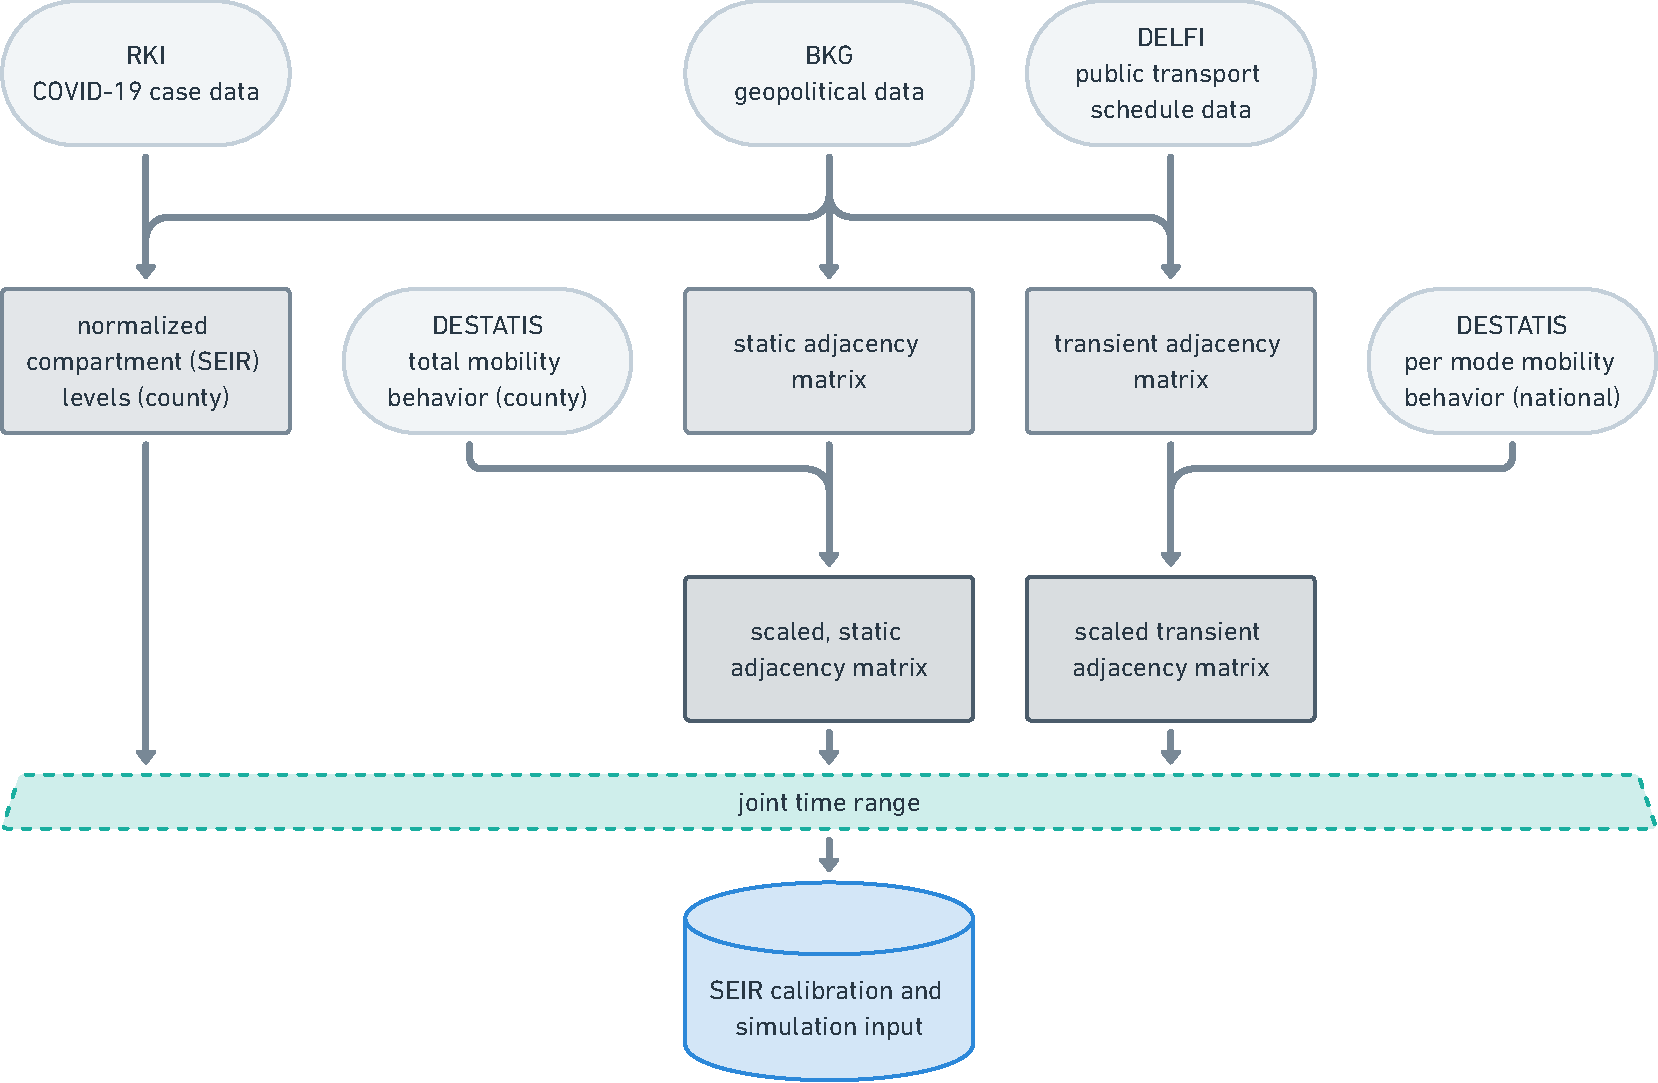
\includegraphics[width=\linewidth]{img/FP_data-pipeline.pdf}
\caption{Data processing pipeline}
  \label{img:flwData}
\end{figure}

\subsubsection{Transient adjacency matrix calculation}\label{ssec:transientAdjancencyMatrixCalculation}
The main body of work of this report is the new method to derive the transient adjacency matrix $A3$ from publicly available data in a programmatic way. The entry point for this calculation is the public transport schedule data collected by a project from DELFI e.V. \cite{delfie.v.OpenDataOPNV2021}. The data sets contain data on schedules of regional and national agencies operating across all of Germany. As the schedule data's intended use is traveling and routing services, the locations are not related to the geopolitical entity county used in this work. Hence, the coordinate information of each stop is tested against the shape information of all counties, which is retrieved from \cite{Verwaltungsgebiete2500002020}. This allows to map stops to counties and subsequently calculate the adjacency matrix as the aggregated number of services between two counties.

To prepare the data set--which is provided in the standard GTFS format--for the calculation of the transient adjacency matrix, the following steps on the respective files are required in the mentioned order:

\begin{enumerate}
	\item agency.txt: reduce to agencies of interest
	\item routes.txt: reduce to routes matching the filtered agency list
	\item trips.txt: reduce to trips matching the route\_id occurrences of the filtered routes list
	\item stop\_times.txt: reduce to stop times matching the filtered trips list
	\item stops.txt: reduce to stop\_id values occurring in the filtered stop times list
	\item calendar: reduce to service\_id values matching the filtered trips list
	\item calendar\_dates.txt: reduce to service\_id values matching the filtered trips list
	\item stops.txt: match latitude and longitude with county polygon from BKG county data and augment stops table with ARS code per stop\footnote{The matching of latitude/longitude tuples with county polygons applies the MATLAB interior point check function iteratively. See \url{https://www.mathworks.com/help/matlab/ref/delaunaytriangulation.isinterior.html}}
	\item stop\_times.txt: augment stop\_times table with ARS code per stop event with the stop\_id $\rightarrow$ ARS mapping of the augmented stops table
\end{enumerate}

Based on the processed schedule data and the successful mapping of stop locations to county codes, the adjacency matrix can finally be calculated as follows:

\begin{enumerate}
	\item combine calendar (cyclic schedule) and calendar\_dates (exceptions) tables to calculate the operation status of each service\_id for the complete time period
	\item iterate over all trips to yield a vector of ARS codes indicating the location of the stops along a trip and use the accompanying service\_id to increment the mobility level for all ARS codes (counties) for every day, where this service\_id is operated
	\item normalize the data\footnote{Unfortunately, the schedule data does not provide information on the capacity of a given vehicle or service event. Similarly, the author was not able to acquire data sets with actual usage figures of public transport on a vehicle level. The adjacency matrix is therefore normalized to the maximum sum of services per departing county. The actual usage figures are then applied via the scaling factor $\psi_3$. Additionally, two other methods of normalization are implemented but produce inferior results: normalization to maximum service count per day for all counties as done by Vrabac et al. and normalization to the sum of services count per starting county per day, which relates to row-wise normalization and results in row-wise stochastic matrices.}
	\item assemble a joint adjacency matrix of all individual GTFS data sets, considering the most recent data as most useful and output a joint adjacency matrix with daily mobility within counties and in between counties
\end{enumerate}

\subsubsection{Parameters to tailor the SEIR model identification and simulation}
The calculation of the transient adjacency matrix $A3$ can be tailored using the following set of filters to inspect a subset of public transport agencies:
\begin{itemize}
	\item includeAgencyList: a positive list of strings to include in the analysis, e.g. "DB" to include "Deutsche Bahn" operated agencies
	\item excludeAgencyList: a negative list of strings to remove from the analysis, e.g. "Bus" to exclude any bus operating agency
\end{itemize}

The identification of the networked SEIR model and the subsequent simulation and counterfactual simulation can be configured with the following set of parameters:
\begin{itemize}
	\item time delays:
	\begin{itemize}
		\item tLagRemoved: time delay in days to be used for removed compartment estimation based on recovered case data
		\item tLagDeath: time delay in days to be used for removed compartment estimation based on death case data; fatalities are considered in this work contrary to the standard SEIR model approach because COVID-19 lead to significant excess mortality \cite{worldhealthorganizationTrueDeathToll} that the author assumes to exceed any birth rate changes
		\item tLeadExposed: time delay in days by which positive test cases are shifted to estimate the exposed compartment
	\end{itemize}
	\item tSmoothCases: time duration of smoothing for simulation input compartment data
	\item h: sampling time of COVID-19 input data
	\item dateStart: start date of simulation interval (if data is available)
	\item dateEnd: stop date of simulation interval (if data is available)
	\item countiesList: specify a list of ARS codes to simulate with
	\item mobilityLevel: a switch to determine the mobility behavior data to use for adjacency matrix scaling; available options are "nation" using \cite{statistischesbundesamtdestatisVerkehrsmittelImFernverkehr2021}, "county" using \cite{statistischesbundesamtdestatisVeranderungsrateMobilitatGgu2021} and "combined" using both
	\item rPopulation: a threshold of population density to omit any lower-density counties from the analysis
	\item counterfactuals:
	\begin{itemize}
		\item type: a switch to select the type of counterfactual to simulate for, available options are "fixed" (a static level of mobility compared to 2019 levels), "scaled" (a multiple of the recovered mobility behavior) and "cappedTop" (an upper bounded version of the recovered mobility behavior)
		\item value: the value to apply according to the counterfactual method selected with type
	\end{itemize}
\end{itemize}

\section{Evaluation}\label{sec:evaluation}

\subsection{Experimental Results}
Based on the MATLAB implementation, the data sets are processed and the networked SEIR model approach is applied. The results are evaluated from two different perspectives: 1) presentation and interpretation of results (numerically and graphically) for identification and simulation of a networked SEIR model for the complete time period, using combined mobility behavior and comparing the results with and without the use of the transient adjacency matrix and 2) comparison to the original results from \cite{vrabacCapturingEffectsTransportation2020}.

\subsubsection{Networked SEIR model identification and simulation results}
The networked SEIR model using German public transport data and mobility behavior data proves to be a very effective approach to model the COVID-19 outbreak even for the multiple waves that occurred until the time of writing. \autoref{fig:compAggrCombWave0} shows a comparison of the results for the networked SEIR model with and without use of the transient adjacency matrix $A3$ as introduced in \autoref{ssec:transientAdjancencyMatrixCalculation}. The plots show the denormalized data per compartment aggregated over the entire nation. As can be seen, the use of the transient adjacency matrix (subplots \autoref{fig:compAggrCombWave0Exp}, \autoref{fig:compAggrCombWave0Inf} and \autoref{fig:compAggrCombWave0Rem}) drastically improves simulation performance and successfully recovers the second and third outbreak.

To yield these results, the settings according to \autoref{tbl:seirSettings} were applied. The identified parameters and error figures are compared in \autoref{tbl:seirParametersAndError}.

As \autoref{tbl:seirParametersAndError} indicates, including the $A3$ adjacency matrix results in higher error of the normalized compartment, but reduces the error on denormalized levels per compartment. This relates well to the orange curves for the simulated pandemic levels in \autoref{fig:compAggrCombWave0}. The deviation on the normalized data presumably results from the incomplete model of the pandemic based on the mobility data alone, as other factors like policy, weather, virus variants, population structure are neglected in this analysis.

 The deviations of the model from the real outbreak data starting in April 2021 are likely attributable to the onset of vaccinations, which are not accounted for in the SEIR model and reduce the susceptible compartment, therefore reducing the pandemic activity.

Additionally, \autoref{fig:compAggrCombWave0} presents the possibility to simulate counterfactuals and check their impact with the identified model. As the plots suggest, the seemingly simple policy of limiting the railway usage to 50\% of 2019 levels might have reduced the pandemic activity by a large margin\footnote{Final levels of removed compartment: real: $3.7182{\times} 10^6$, simulated: $3.0049{\times} 10^6$, counterfactual: $1.8377{\times} 10^6$}.

\begin{table}[h]
     \centering
     \caption{Settings for the identification and simulation for 01-Feb-2020 to 23-Jun-2021}
     \begin{tabular*}{.75\linewidth}{l||l}
     Option & Value \\
     \hline
     \hline
     tLagRemoved & 7\\
     tLagDeath & 7\\
     tLeadExposed & 7\footnotemark\\
     tSmoothCases & 7\\
     h & 1\\
     mobilityLevel & combined\\
     counterfactual type & cappedTop\\
     counterfactual value & 0.5\\
     \hline
     \end{tabular*}
     \label{tbl:seirSettings}
\end{table}
\footnotetext{The RKI notes a median of 5-6 days and a 95th percentile of 10-14 days incubation period based on a survey of studies. \cite{robertkoch-institutrkiEpidemiologischerSteckbriefSARSCoV22021}}

\begin{table}[h]
     \centering
     \caption[]{Identification results and error metrics\footnotemark of the networked SEIR model for 01-Feb-2020 to 23-Jun-2021}
     \begin{tabular*}{\linewidth}{l||p{3.1cm}|p{3.1cm}}
     Metric & $A3 \neq 0$ & $A3 = 0$ \\
     \hline
     \hline
     $\beta_E$ &$[6.8 {\times} 10^{\shortminus5},\linebreak[1] 0.1354,$\newline$ 0.0574]$ &$[6.3 {\times} 10^{\shortminus8},\linebreak[1] 0.1497,$\newline$ 0]$\\
     $\beta_I$ &$[1.8 {\times} 10^{\shortminus5},\linebreak[1] 7.8 {\times} 10^{\shortminus7},\linebreak[1] 3.3 {\times} 10^{\shortminus4}]$ &$[9 {\times} 10^{-9},\linebreak[1] 2.8 {\times} 10^{\shortminus8},\linebreak[1] 0]$\\
     $\sigma$ &$0.1395$ &$0.1390$\\
     $\gamma$ &$0.1394$ &$0.1392$\\
     $\frac{\lVert e_{real} - e_{sim} \rVert}{\lVert e_{real} \rVert}$ &$1.955, 0.4588$ &$1.132, 0.9379$\\
     $\frac{\lVert i_{real} - i_{sim} \rVert}{\lVert i_{real} \rVert}$ &$2.023, 0.4641$ &$1.130, 0.9379$\\
     $\frac{\lVert r_{real} - r_{sim} \rVert}{\lVert r_{real} \rVert}$ &$2.039, 0.4588$ &$1.076, 0.9457$\\
     \hline
     \end{tabular*}
     \label{tbl:seirParametersAndError}
\end{table}
\footnotetext{Two error metrics are presented per compartment. The first one is calculated on normalized compartment levels, while the second one is calculated on aggregated, denormalized levels.}
    
\begin{figure}[hbtp]
     \centering
     \begin{subfigure}[b]{.45\linewidth}
         \centering
         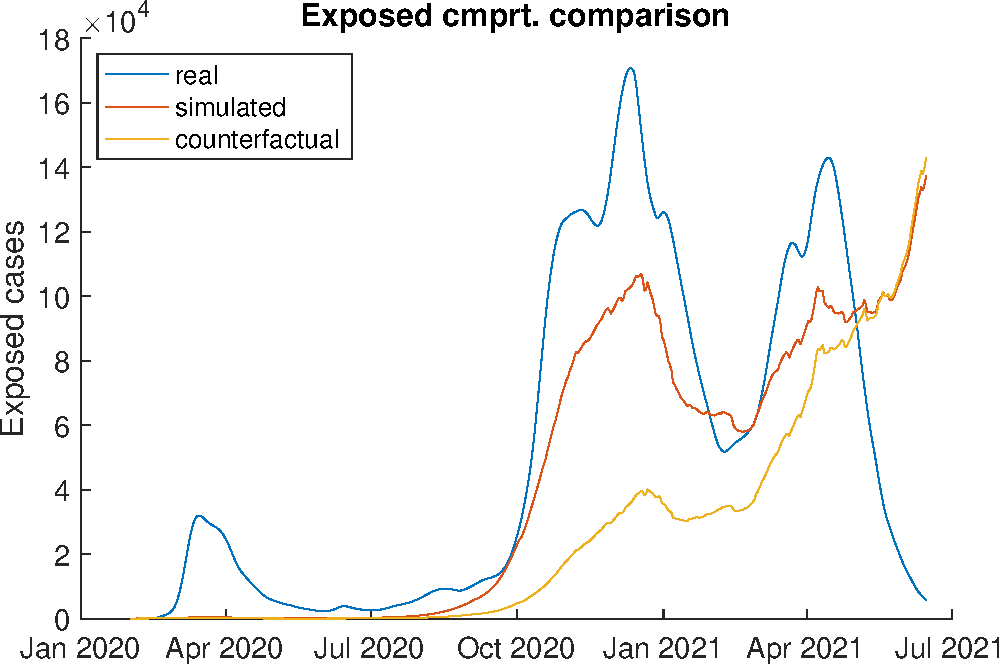
\includegraphics[width=\linewidth]{img/210907_171119_combined_wave0/figures/COMP_exp}
         \caption{Exposed, $A3 \neq 0$}
         \label{fig:compAggrCombWave0Exp}
     \end{subfigure}
     \hfill
     \begin{subfigure}[b]{.45\linewidth}
         \centering
         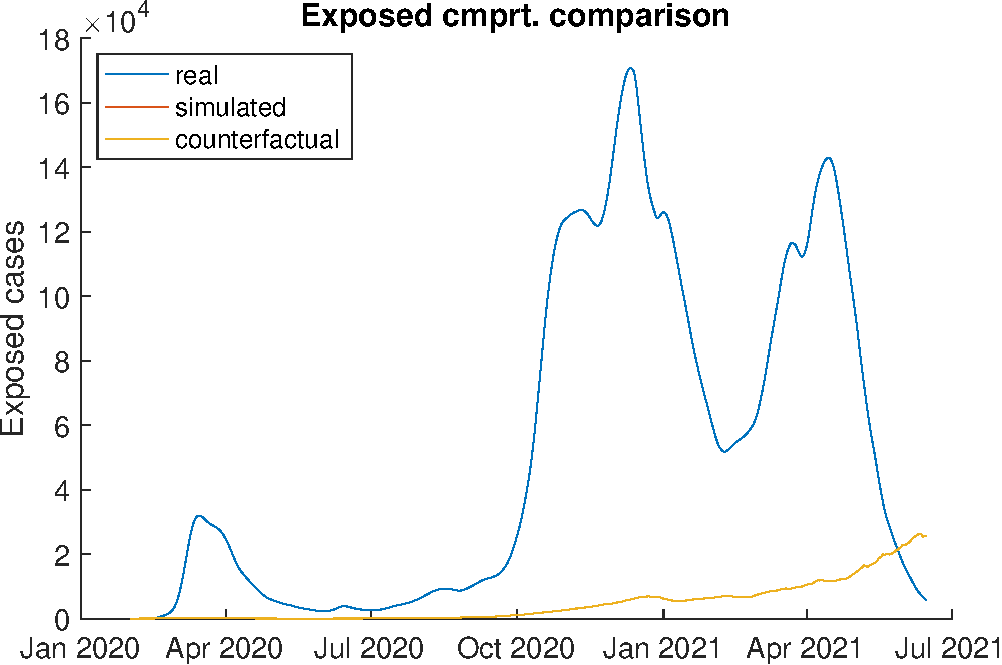
\includegraphics[width=\linewidth]{img/210907_180927_combined_wave0_noa3/figures/COMP_exp}
         \caption{Exposed, $A3 = 0$}
         \label{fig:compAggrCombWave0NoA3Exp}
     \end{subfigure}
     \newline
     \begin{subfigure}[b]{.45\linewidth}
         \centering
         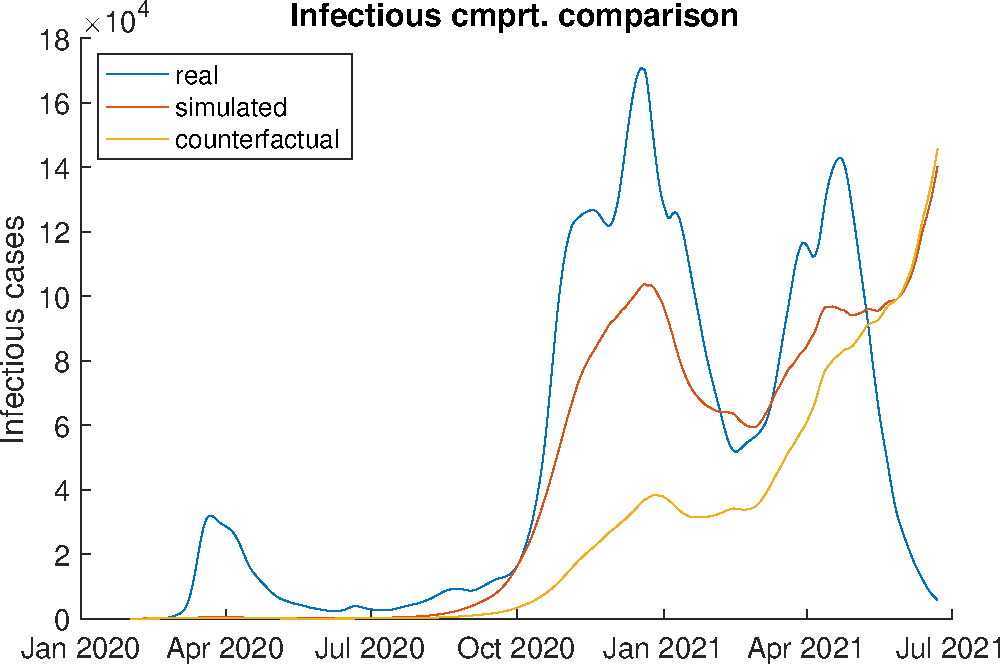
\includegraphics[width=\linewidth]{img/210907_171119_combined_wave0/figures/COMP_inf}
         \caption{Infectious, $A3 \neq 0$}
         \label{fig:compAggrCombWave0Inf}
     \end{subfigure}
     \hfill
     \begin{subfigure}[b]{.45\linewidth}
         \centering
         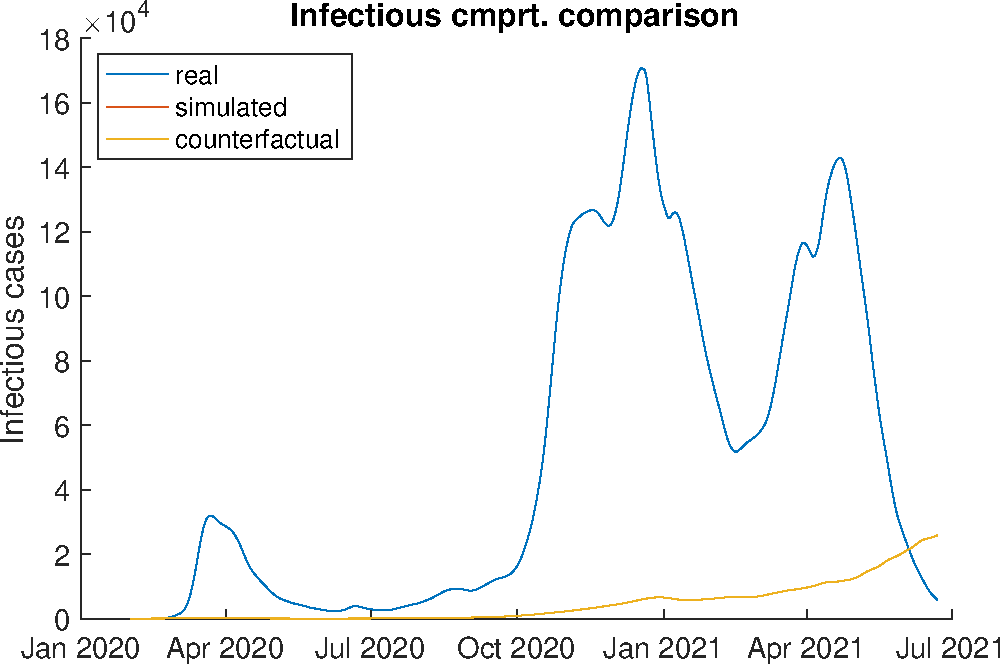
\includegraphics[width=\linewidth]{img/210907_180927_combined_wave0_noa3/figures/COMP_inf}
         \caption{Infectious, $A3 = 0$}
         \label{fig:compAggrCombWave0NoA3Inf}
     \end{subfigure}
     \newline
     \begin{subfigure}[b]{.45\linewidth}
         \centering
         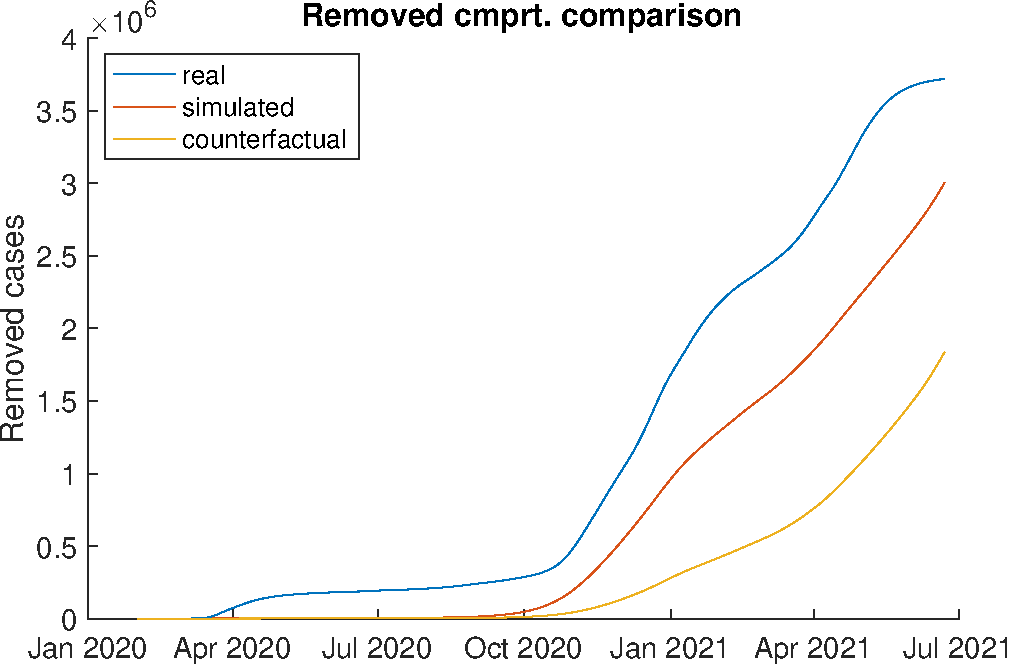
\includegraphics[width=\linewidth]{img/210907_171119_combined_wave0/figures/COMP_rem}
         \caption{Removed, $A3 \neq 0$}
         \label{fig:compAggrCombWave0Rem}
     \end{subfigure}
     \hfill
     \begin{subfigure}[b]{.45\linewidth}
         \centering
         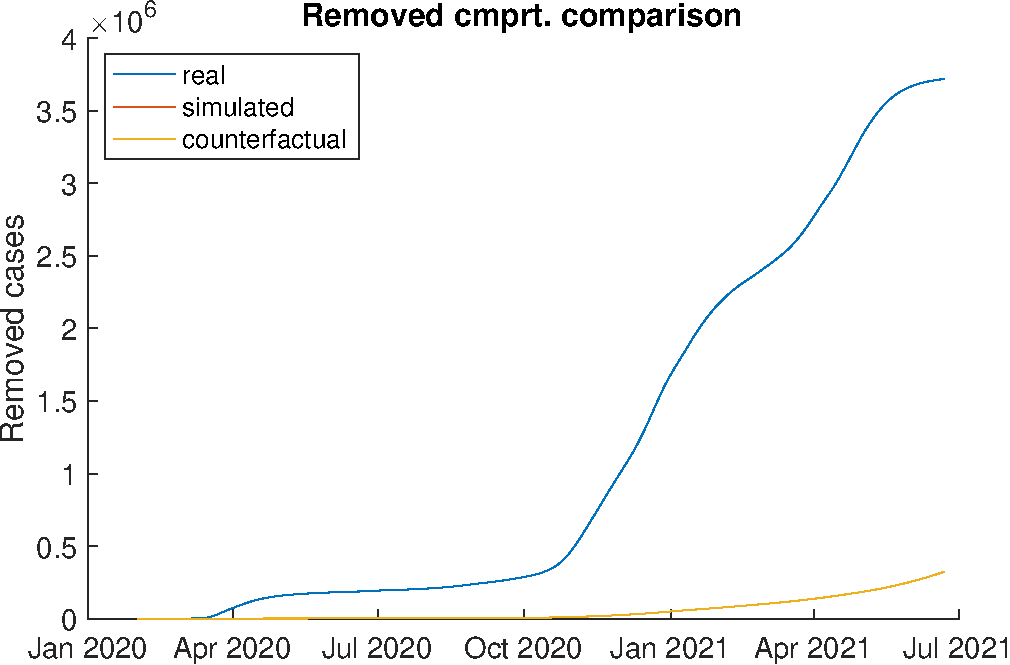
\includegraphics[width=\linewidth]{img/210907_180927_combined_wave0_noa3/figures/COMP_rem}
         \caption{Removed, $A3 = 0$}
         \label{fig:compAggrCombWave0NoA3Rem}
     \end{subfigure}     
     \caption[Comparison of aggregated, denormalized compartment levels of networked SEIR model with and without $A3$]{Comparison of aggregated, denormalized compartment levels of networked SEIR model with and without $A3$\protect\footnotemark}
     \label{fig:compAggrCombWave0}
\end{figure}
\footnotetext{The counterfactual line represents the outcome of a theoretical change in the usage behavior of public transport. The plots show the results of applying upper bounded ($50 \%$) behavior data as $\psi_{3_j}$. The simulated and counterfactual lines intersect for subplots (b), (d) and (f) as $A3=0$.}

\subsubsection{Comparison to the results of Vrabac et al.}
This work differs to the approach and results presented in \cite{vrabacCapturingEffectsTransportation2020} in the following categories:

\begin{itemize}
	\item The scope of analysis is the entire set of counties of Germany instead of a subset of counties from the U.S.
	\item The time range includes not just the first COVID-19 outbreak but considers all three waves that occurred until the time of writing.
	\item The scaling of the adjacency matrix is performed based on measured mobility behavior--which correlates with policy information--instead of guessed parameters.
	\item The analysis is validated against denormalized data.
\end{itemize}

\section{Discussion}
The new approach to pandemic modeling based on networked entities represented by adjacency matrices that are programmatically calculated based on official data from government agencies shows good performance for recovery and prediction of the pandemic activity on the nation level.

As was shown, the small number of parameters depicted in \autoref{tbl:seirSettings} is sufficient to tailor the framework. At the same time, different data can be easily included for identification and simulation with the networked SEIR model by extending the behavior/policy factors $\psi$. Both aspects allow to consider other data sources for COVID-19 simulation or modify the framework to apply it to other epidemics.

Still, \autoref{fig:compAggrCombWave0} and the plots in \autoref{sec:variationsOfSEIRSettings} show that the approach presented herein does not model the COVID-19 outbreak either completely or reliably. This is partly caused by neglected effects\footnote{Vaccinations are not considered and mandate the introduction of a new compartment with transitions from susceptible to vaccinated. Additionally, new studies show that neither recovered nor fully vaccinated people exhibit permanent protection from infections. Hence, a SEIRS model as proposed \cite{bjornstadSEIRSModelInfectious2020} with a transition from removed to susceptible should be investigated.}, but also likely influenced by underreporting of cases causing a wrong estimation of the actual pandemic levels. It is further affected by time-varying test policy and number of tests executed--and subsequently positive test ratios--as well as official COVID-19 legislation and varying spread characteristics of the different SARS-CoV-2 virus strains--though the spread supporting factors are still under investigation.

\subsection{Sensitivity Analysis}
An extensive sensitivity analysis was not performed due to the large size of the data sets and the extensive set of parameters and settings. Nevertheless, a number of different scopes of analysis and their impact is presented in \autoref{sec:variationsOfSEIRSettings}.
\section{Conclusion}
To conclude, the networked SEIR model from \cite{vrabacCapturingEffectsTransportation2020} was applied to German geopolitical, transport and behavior data. The experimental results suggest that mobility induced spreading is an important factor, though community spreading within counties still accounts for the majority of transmission (see \autoref{tbl:seirParametersAndError} and \cite{aravindakshanPreparingFutureCOVID192020}). Counterfactual simulation with a modified behavior vector suggests that reduced long-distance rail-bound mobility played a role in reducing the pandemic spread and could be a measure to contain future outbreaks. Future works building on the approach should consider a) addition of a new compartment for vaccinated cases alongside declined immunity over time \cite{bjornstadSEIRSModelInfectious2020} and b) introduction of novel data sources like policy information, weather data or virus strain characteristics to improve the scaling factors $\psi$ of the adjacency matrices for further improvement of the model's accuracy.


%%%%%%%%%%%%%%%%%%%%%%%%%%%%% APPENDIX %%%%%%%%%%%%%%%%%%%%%%%%%%%%%%%%
% APPENDIX
%\appendix
\appendices
\section{Variation of settings of the networked SEIR model identification and simulation}\label{sec:variationsOfSEIRSettings}
This section presents the impact of different time ranges on the results of the parameter identification and subsequent simulation. To provide a better understanding of the effects of the options on the behavior of the networked SEIR model, both the aggregated, denormalized compartment levels and the normalized compartment levels per county are presented. As can be seen, aggregated levels are more consistent with the real pandemic activity, while the spread levels of the individual counties show large deviations resulting from this work's focus on the mobility behavior of the population and suggesting to consider additional data for the scaling factors $\psi$.

\subsection{Wave 1 - from 01-FEB-2020 to 01-SEP-2020}

\autoref{fig:compCombWave1} shows how the networked SEIR model fails to recover the spread activity for wave 1. The root cause is unknown, but indicates, that mobility is only one of the many drivers of a pandemic.

\begin{figure}[hbtp]
     \centering
     \begin{subfigure}[b]{.45\linewidth}
         \centering
         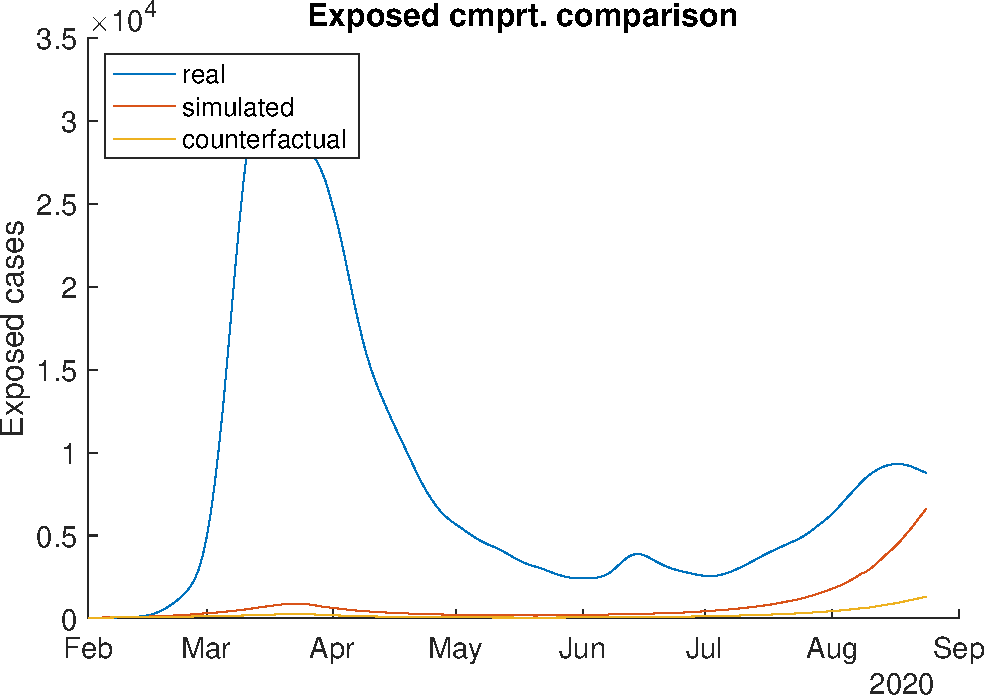
\includegraphics[width=\linewidth]{img/210907_221615_combined_wave1/figures/COMP_exp}
         \caption{Exposed}
         \label{fig:compAggrCombWave1Exp}
     \end{subfigure}
     \hfill
     \begin{subfigure}[b]{.45\linewidth}
         \centering
         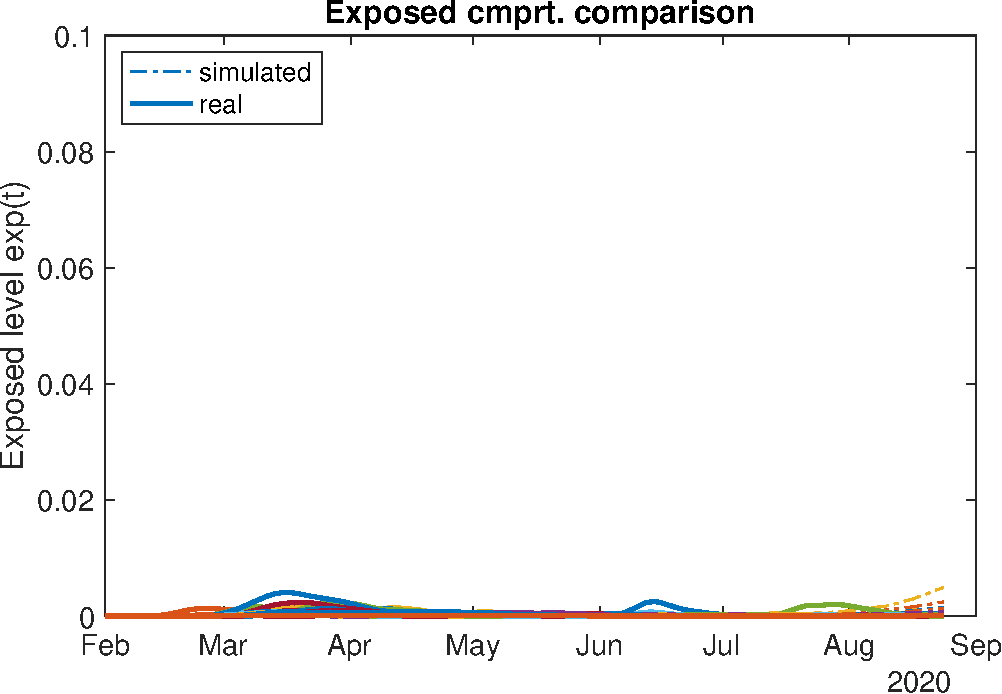
\includegraphics[width=\linewidth]{img/210907_221615_combined_wave1/figures/SEIR_e_sim-vs-real}
         \caption{Exposed}
         \label{fig:compCombWave1Exp}
     \end{subfigure}
     \newline
     \begin{subfigure}[b]{.45\linewidth}
         \centering
         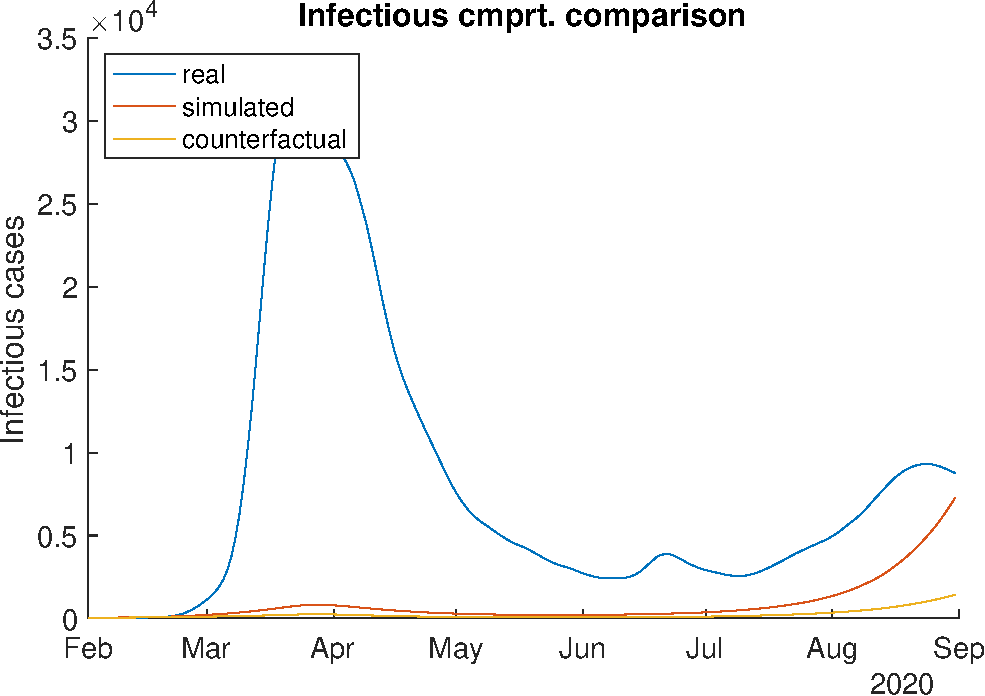
\includegraphics[width=\linewidth]{img/210907_221615_combined_wave1/figures/COMP_inf}
         \caption{Infectious}
         \label{fig:compAggrCombWave1Inf}
     \end{subfigure}
     \hfill
     \begin{subfigure}[b]{.45\linewidth}
         \centering
         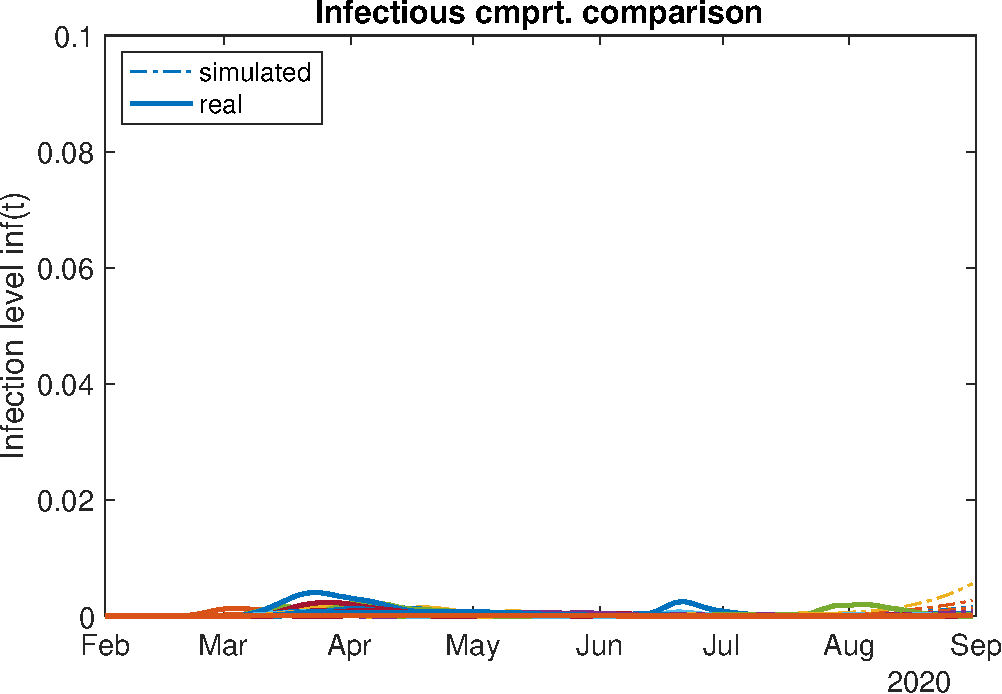
\includegraphics[width=\linewidth]{img/210907_221615_combined_wave1/figures/SEIR_i_sim-vs-real}
         \caption{Infectious}
         \label{fig:compCombWave1Inf}
     \end{subfigure}
     \newline
     \begin{subfigure}[b]{.45\linewidth}
         \centering
         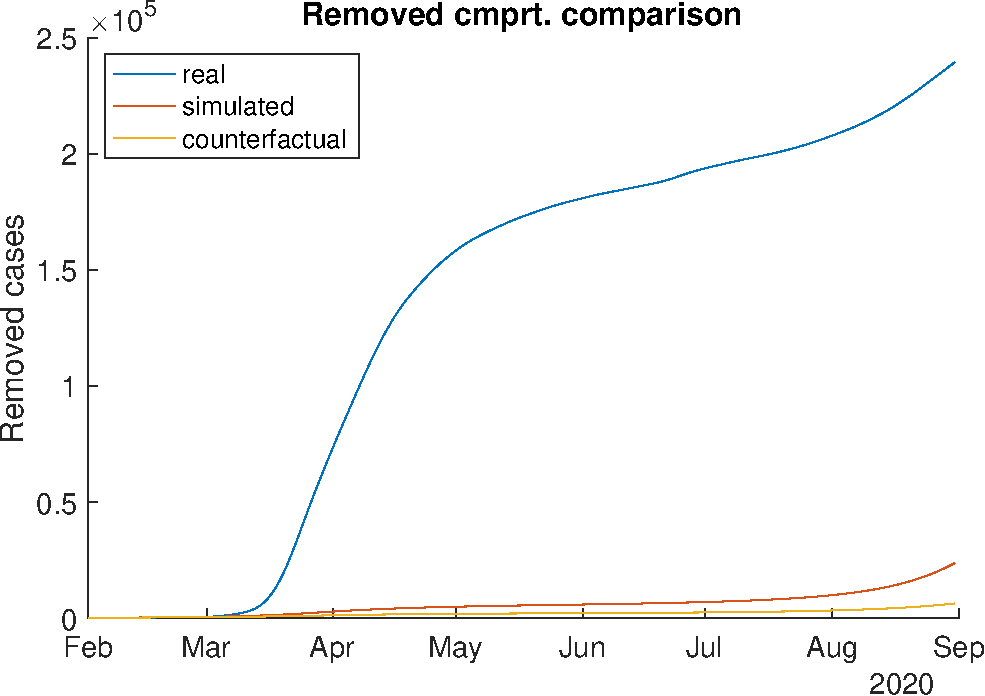
\includegraphics[width=\linewidth]{img/210907_221615_combined_wave1/figures/COMP_rem}
         \caption{Removed}
         \label{fig:compAggrCombWave1Rem}
     \end{subfigure}
     \hfill
     \begin{subfigure}[b]{.45\linewidth}
         \centering
         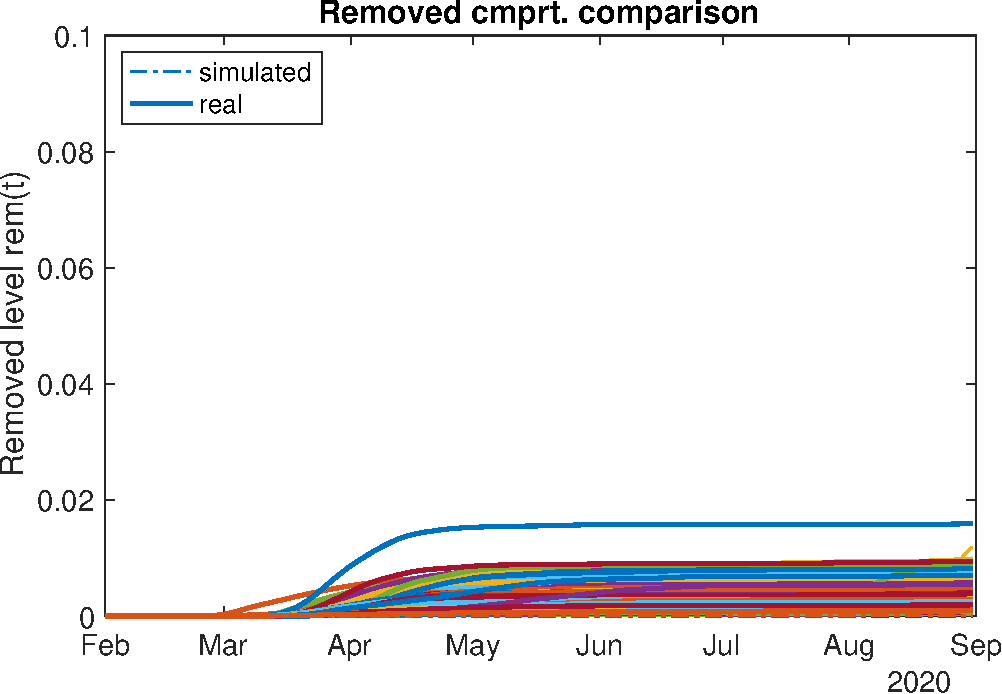
\includegraphics[width=\linewidth]{img/210907_221615_combined_wave1/figures/SEIR_r_sim-vs-real}
         \caption{Removed}
         \label{fig:compCombWave1Rem}
     \end{subfigure}     
     \caption{Compartment levels, wave 1 with combined mobility; left: normalized per county, right: aggregated denormalized}
     \label{fig:compCombWave1}
\end{figure}

\subsection{Wave 2 - from 01-SEP-2020 to 15-MAR-2021}

\autoref{fig:compCombWave2} is a good example of the performance of the networked SEIR model. As can be seen, the simulated behavior is matching the real behavior both in time and magnitude of the outbreak. The counterfactual shows similar reduction in pandemic activity as was shown for the complete time period in \autoref{sec:evaluation}.

\begin{figure}[hbtp]
     \centering
     \begin{subfigure}[b]{.45\linewidth}
         \centering
         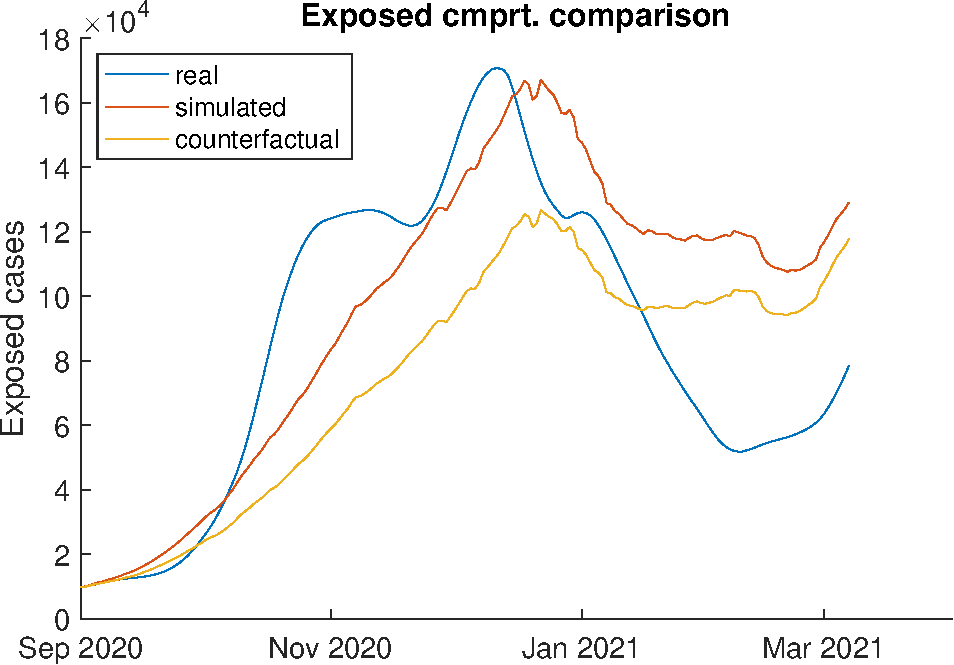
\includegraphics[width=\linewidth]{img/210907_223108_combined_wave2/figures/COMP_exp}
         \caption{Exposed}
         \label{fig:compAggrCombWave2Exp}
     \end{subfigure}
     \hfill
     \begin{subfigure}[b]{.45\linewidth}
         \centering
         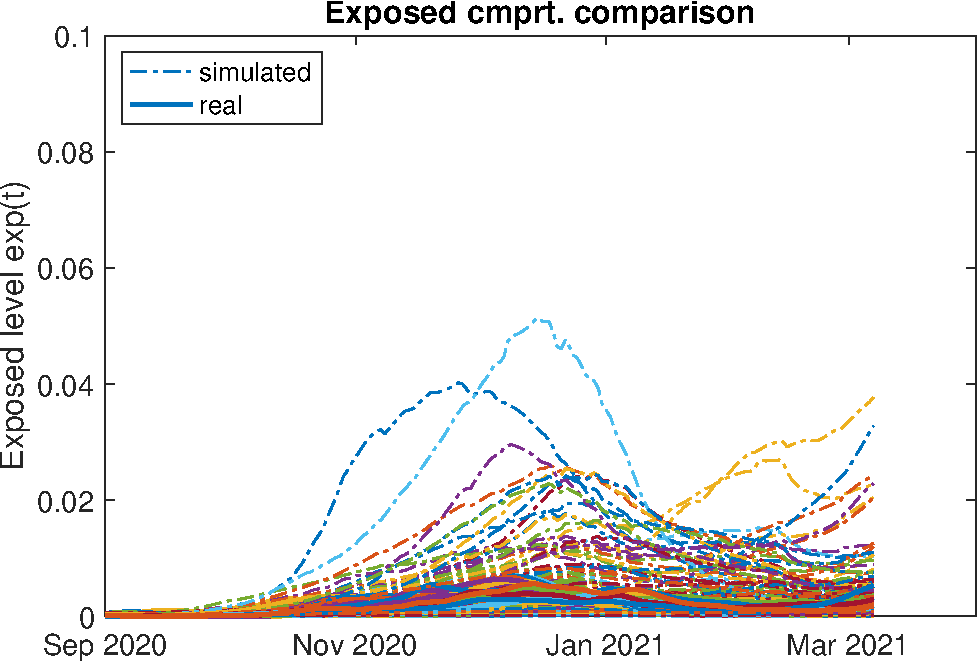
\includegraphics[width=\linewidth]{img/210907_223108_combined_wave2/figures/SEIR_e_sim-vs-real}
         \caption{Exposed}
         \label{fig:compCombWave2Exp}
     \end{subfigure}
     \newline
     \begin{subfigure}[b]{.45\linewidth}
         \centering
         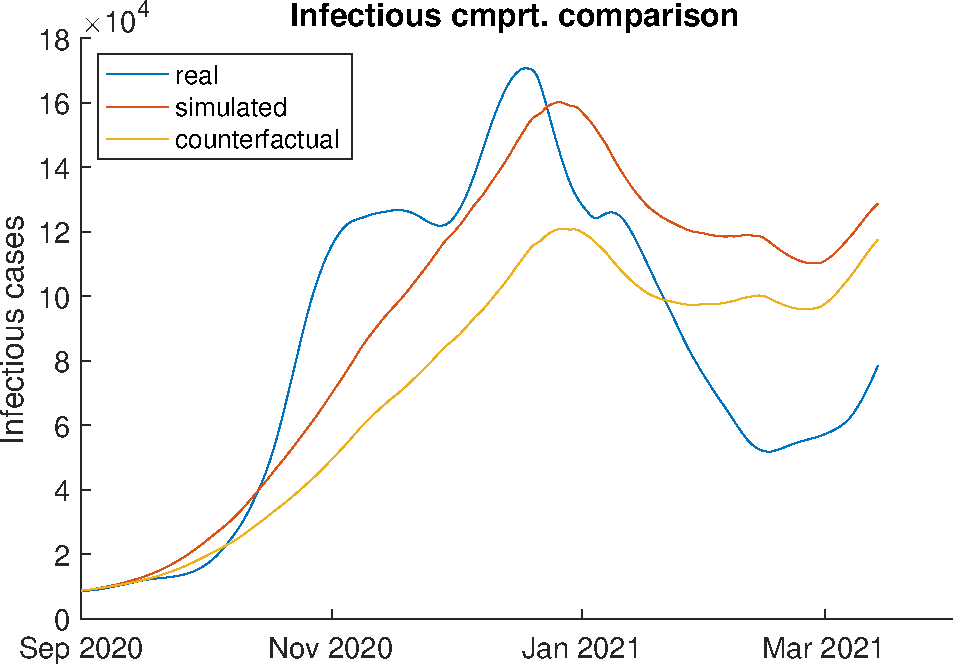
\includegraphics[width=\linewidth]{img/210907_223108_combined_wave2/figures/COMP_inf}
         \caption{Infectious}
         \label{fig:compAggrCombWave2Inf}
     \end{subfigure}
     \hfill
     \begin{subfigure}[b]{.45\linewidth}
         \centering
         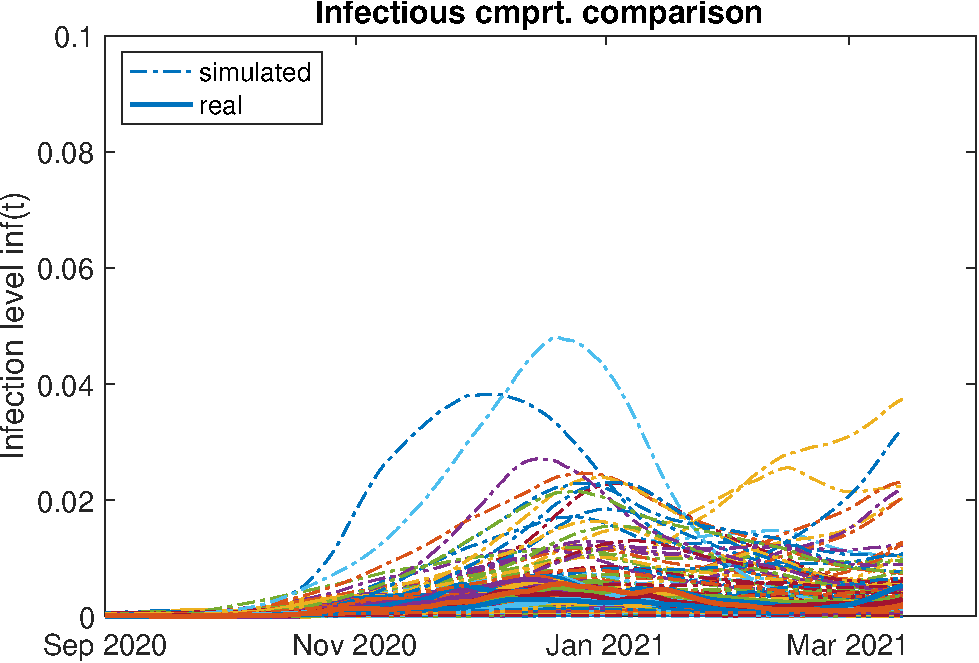
\includegraphics[width=\linewidth]{img/210907_223108_combined_wave2/figures/SEIR_i_sim-vs-real}
         \caption{Infectious}
         \label{fig:compCombWave2Inf}
     \end{subfigure}
     \newline
     \begin{subfigure}[b]{.45\linewidth}
         \centering
         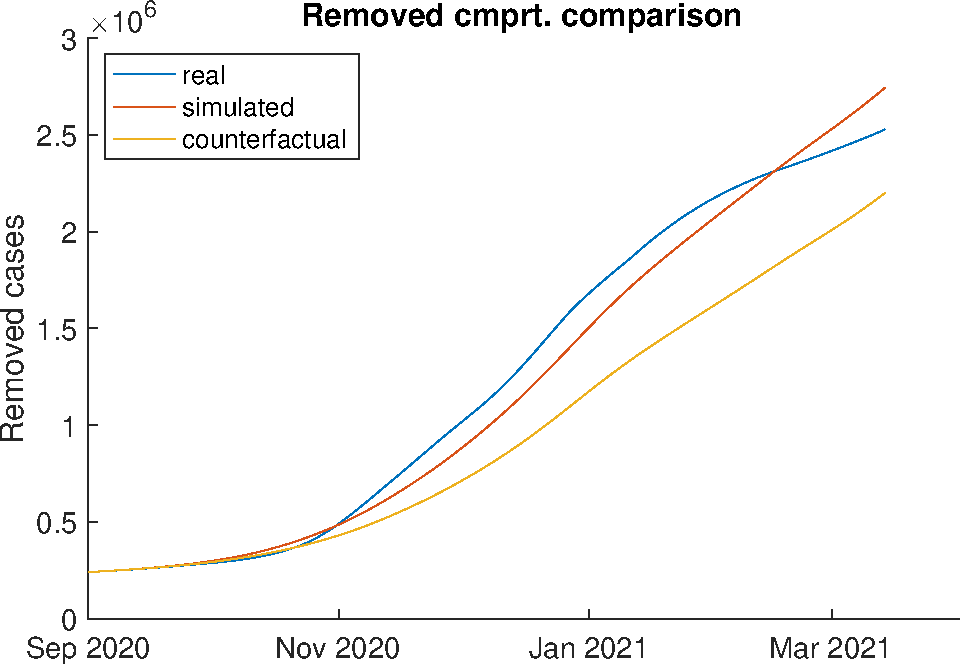
\includegraphics[width=\linewidth]{img/210907_223108_combined_wave2/figures/COMP_rem}
         \caption{Removed}
         \label{fig:compAggrCombWave2Rem}
     \end{subfigure}
     \hfill
     \begin{subfigure}[b]{.45\linewidth}
         \centering
         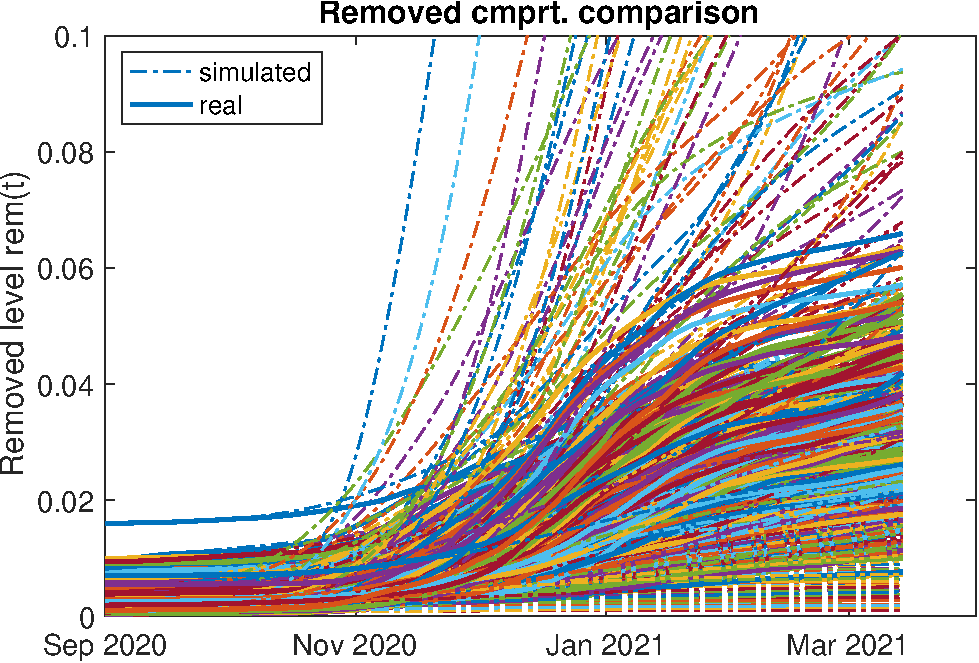
\includegraphics[width=\linewidth]{img/210907_223108_combined_wave2/figures/SEIR_r_sim-vs-real}
         \caption{Removed}
         \label{fig:compCombWave2Rem}
     \end{subfigure}     
     \caption{Compartment levels, wave 2 with combined mobility; left: normalized per county, right: aggregated denormalized}
     \label{fig:compCombWave2}
\end{figure}

\subsection{Wave 3 - from 15-MAR-2021 to 23-JUN-2021}

The analysis of the third wave in \autoref{fig:compCombWave3} is a powerful example for the shortcomings of the approach. The plots clearly show that the simulation is not able to match the actual, measured spread activity and instead predicts an almost constant level of infections--though yielding similar removed compartment levels. This suggests to consider a new compartment for vaccinated cases, as the observed decline of real cases likely results from a decrease in the susceptible compartment due to the success of the vaccination program.

\begin{figure}[hbtp]
     \centering
     \begin{subfigure}[b]{.45\linewidth}
         \centering
         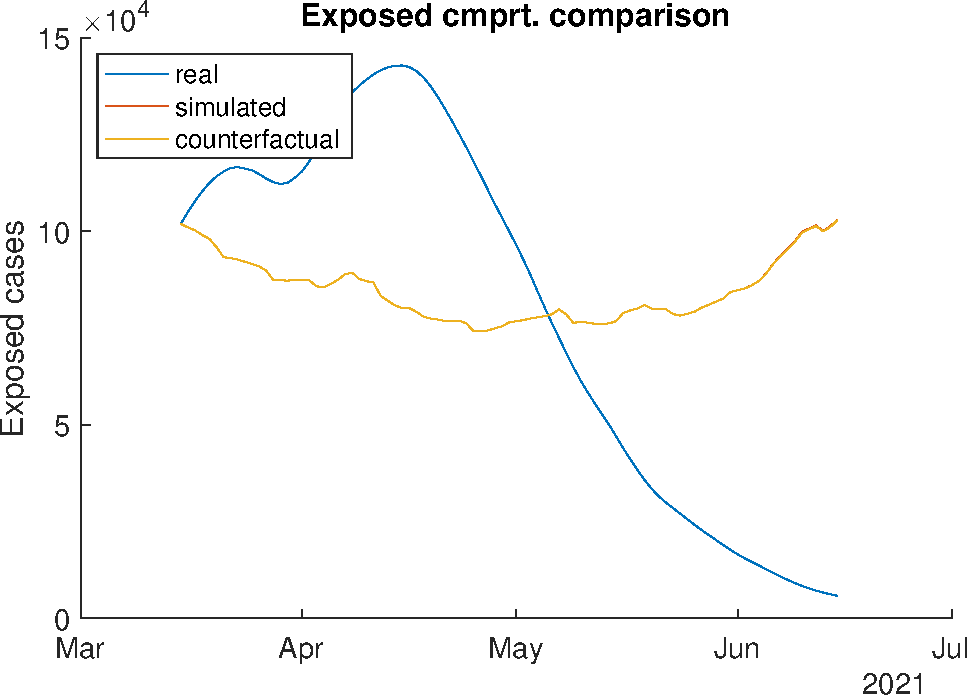
\includegraphics[width=\linewidth]{img/210907_224100_combined_wave3/figures/COMP_exp}
         \caption{Exposed}
         \label{fig:compAggrCombWave3Exp}
     \end{subfigure}
     \hfill
     \begin{subfigure}[b]{.45\linewidth}
         \centering
         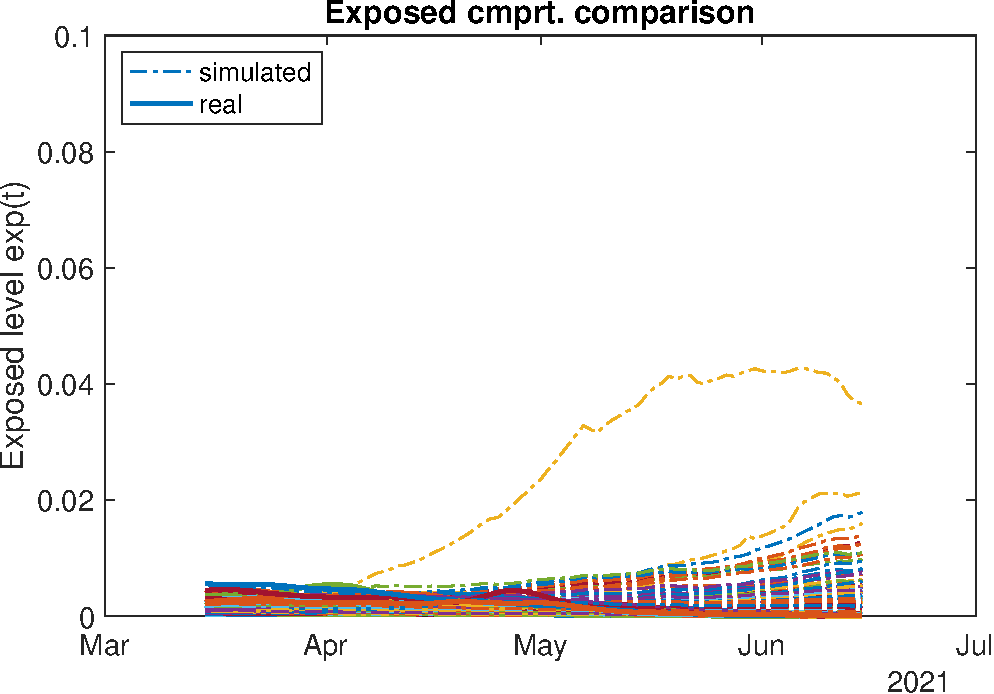
\includegraphics[width=\linewidth]{img/210907_224100_combined_wave3/figures/SEIR_e_sim-vs-real}
         \caption{Exposed}
         \label{fig:compCombWave3Exp}
     \end{subfigure}
     \newline
     \begin{subfigure}[b]{.45\linewidth}
         \centering
         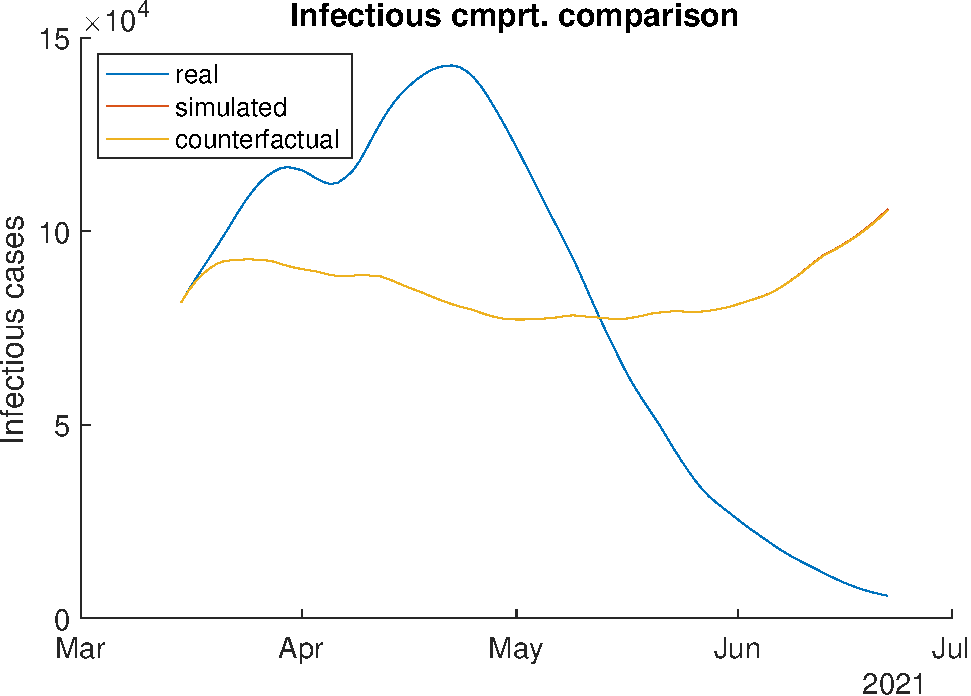
\includegraphics[width=\linewidth]{img/210907_224100_combined_wave3/figures/COMP_inf}
         \caption{Infectious}
         \label{fig:compAggrCombWave3Inf}
     \end{subfigure}
     \hfill
     \begin{subfigure}[b]{.45\linewidth}
         \centering
         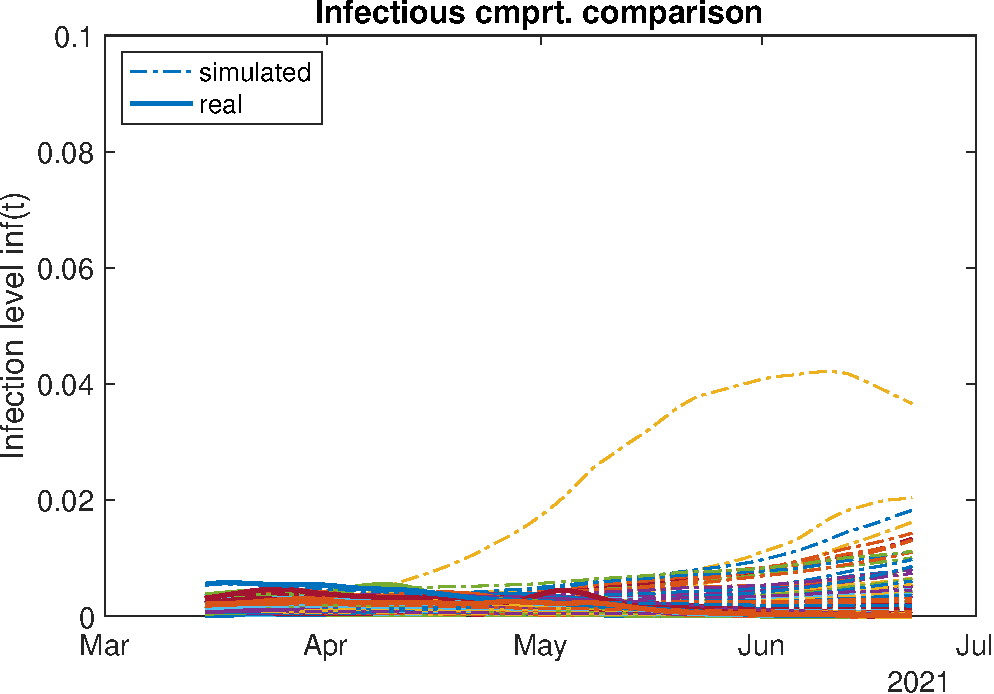
\includegraphics[width=\linewidth]{img/210907_224100_combined_wave3/figures/SEIR_i_sim-vs-real}
         \caption{Infectious}
         \label{fig:compCombWave3Inf}
     \end{subfigure}
     \newline
     \begin{subfigure}[b]{.45\linewidth}
         \centering
         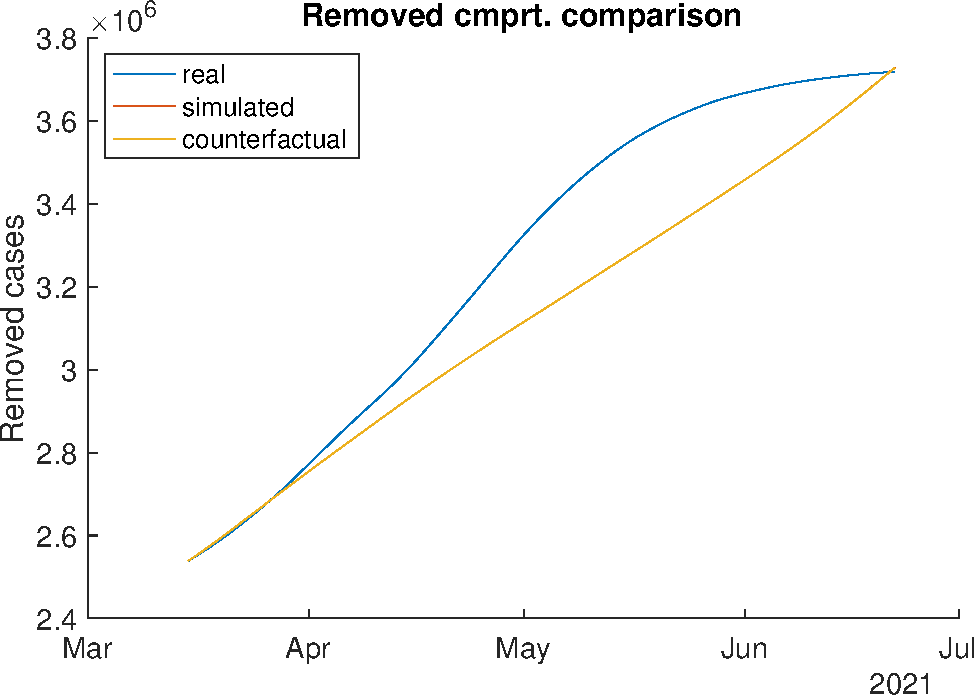
\includegraphics[width=\linewidth]{img/210907_224100_combined_wave3/figures/COMP_rem}
         \caption{Removed}
         \label{fig:compAggrCombWave3Rem}
     \end{subfigure}
     \hfill
     \begin{subfigure}[b]{.45\linewidth}
         \centering
         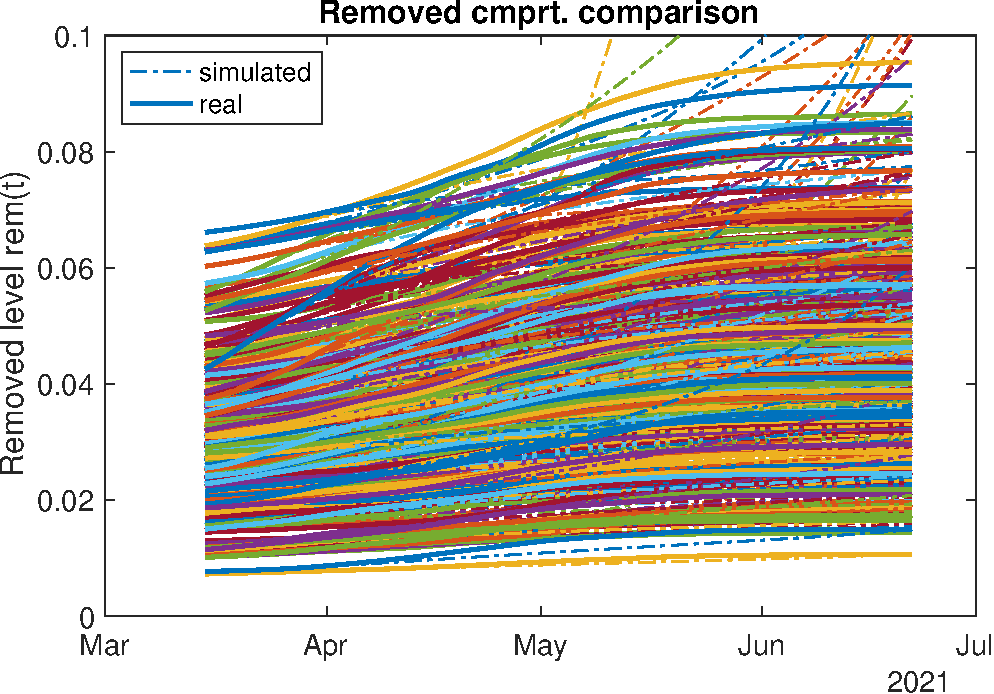
\includegraphics[width=\linewidth]{img/210907_224100_combined_wave3/figures/SEIR_r_sim-vs-real}
         \caption{Removed}
         \label{fig:compCombWave3Rem}
     \end{subfigure}     
     \caption{Compartment levels, wave 3 with combined mobility; left: normalized per county, right: aggregated denormalized}
     \label{fig:compCombWave3}
\end{figure}

\subsection{Waves 2 and 3 - from 01-SEP-2021 to 23-JUN-2021}

The combined analysis of the second and third wave in \autoref{fig:compCombWave23} shows a similar behavior as presented in \autoref{sec:evaluation} except for the huge deviations fore the omitted first wave. The plots support the networked SEIR model's ability to recover the two distinct waves purely from the measured mobility behavior of the population under analysis.

\begin{figure}[hbtp]
     \centering
     \begin{subfigure}[b]{.45\linewidth}
         \centering
         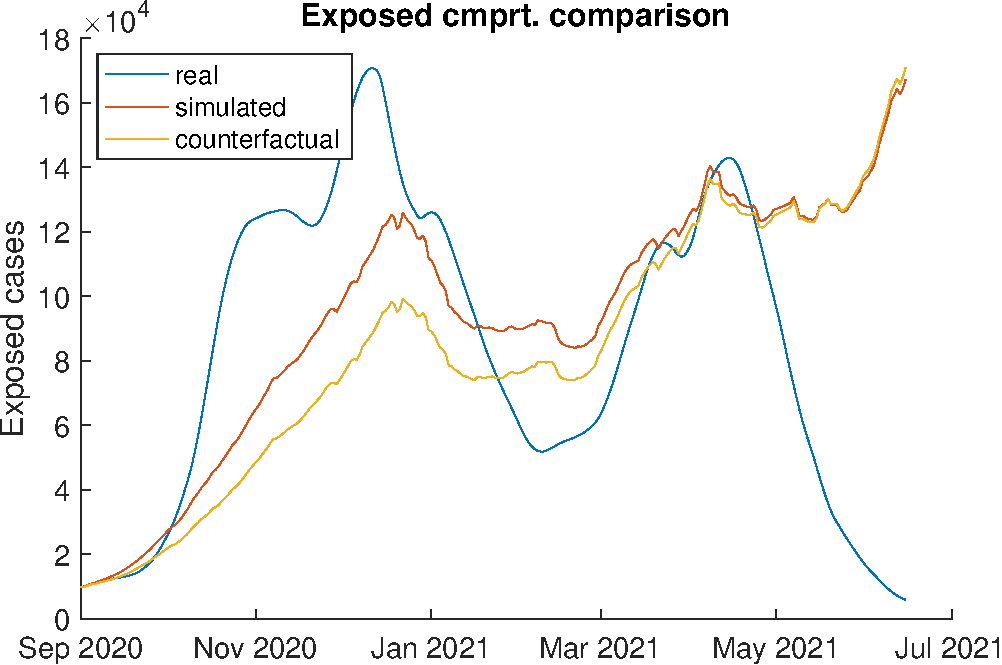
\includegraphics[width=\linewidth]{img/210907_224622_combined_wave23/figures/COMP_exp}
         \caption{Exposed}
         \label{fig:compAggrCombWave23Exp}
     \end{subfigure}
     \hfill
     \begin{subfigure}[b]{.45\linewidth}
         \centering
         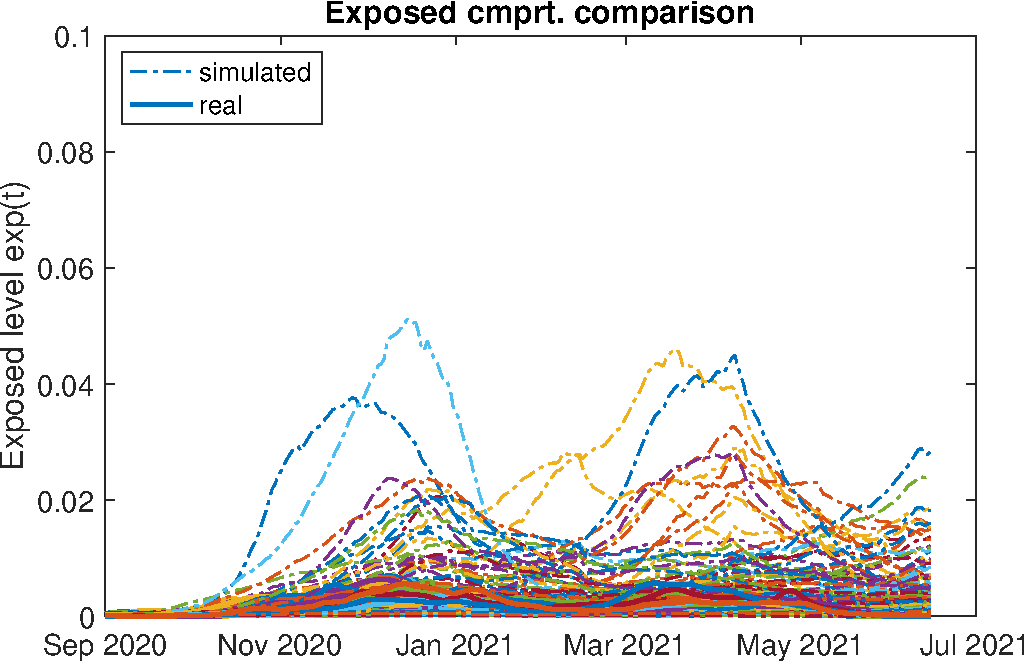
\includegraphics[width=\linewidth]{img/210907_224622_combined_wave23/figures/SEIR_e_sim-vs-real}
         \caption{Exposed}
         \label{fig:compCombWave23Exp}
     \end{subfigure}
     \newline
     \begin{subfigure}[b]{.45\linewidth}
         \centering
         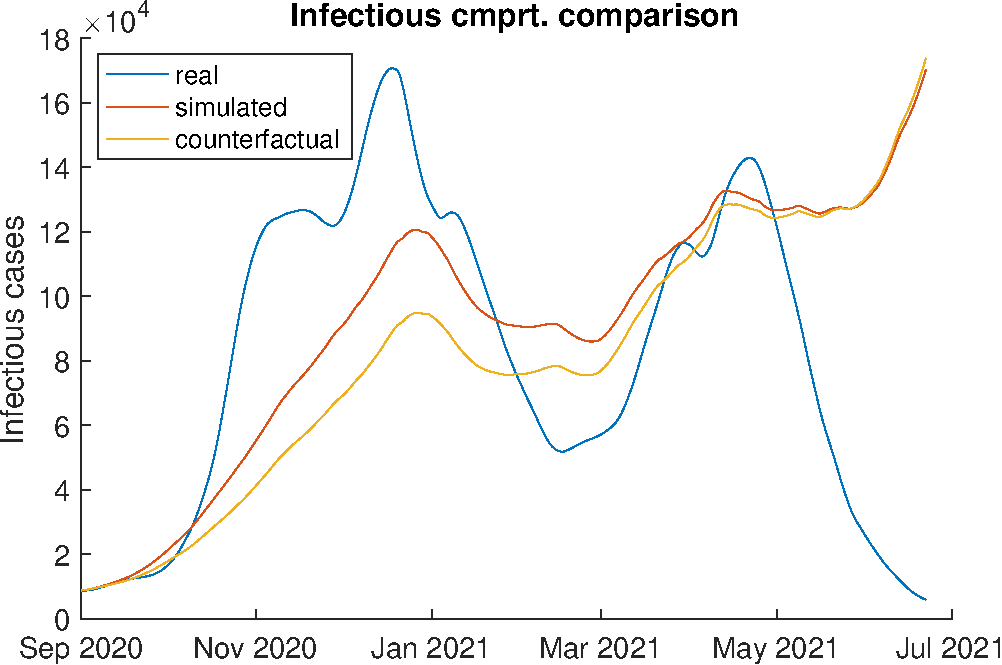
\includegraphics[width=\linewidth]{img/210907_224622_combined_wave23/figures/COMP_inf}
         \caption{Infectious}
         \label{fig:compAggrCombWave23Inf}
     \end{subfigure}
     \hfill
     \begin{subfigure}[b]{.45\linewidth}
         \centering
         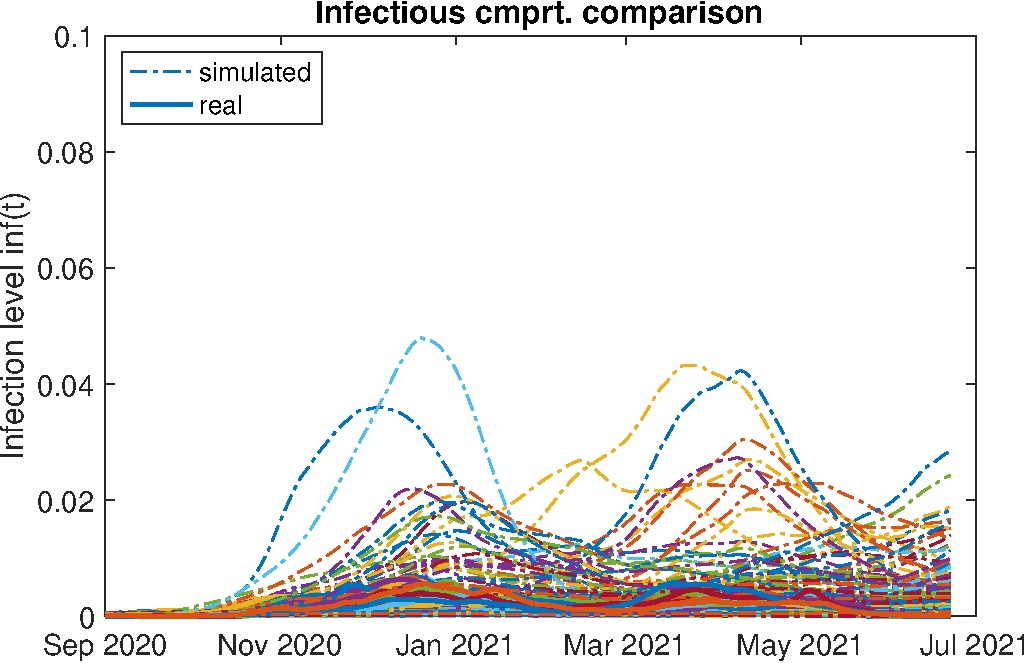
\includegraphics[width=\linewidth]{img/210907_224622_combined_wave23/figures/SEIR_i_sim-vs-real}
         \caption{Infectious}
         \label{fig:compCombWave23Inf}
     \end{subfigure}
     \newline
     \begin{subfigure}[b]{.45\linewidth}
         \centering
         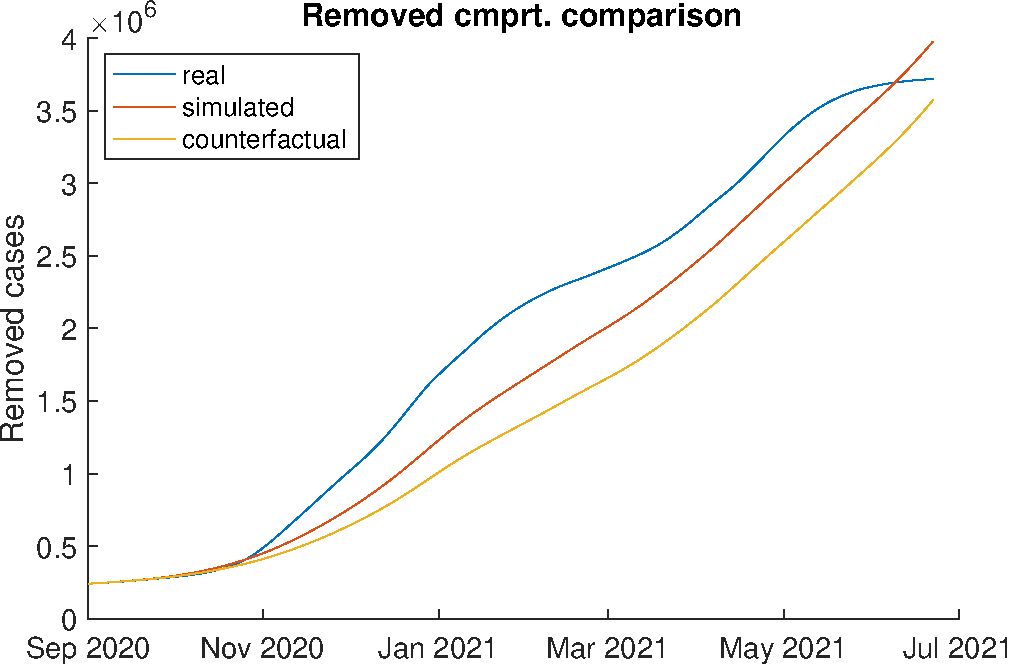
\includegraphics[width=\linewidth]{img/210907_224622_combined_wave23/figures/COMP_rem}
         \caption{Removed}
         \label{fig:compAggrCombWave23Rem}
     \end{subfigure}
     \hfill
     \begin{subfigure}[b]{.45\linewidth}
         \centering
         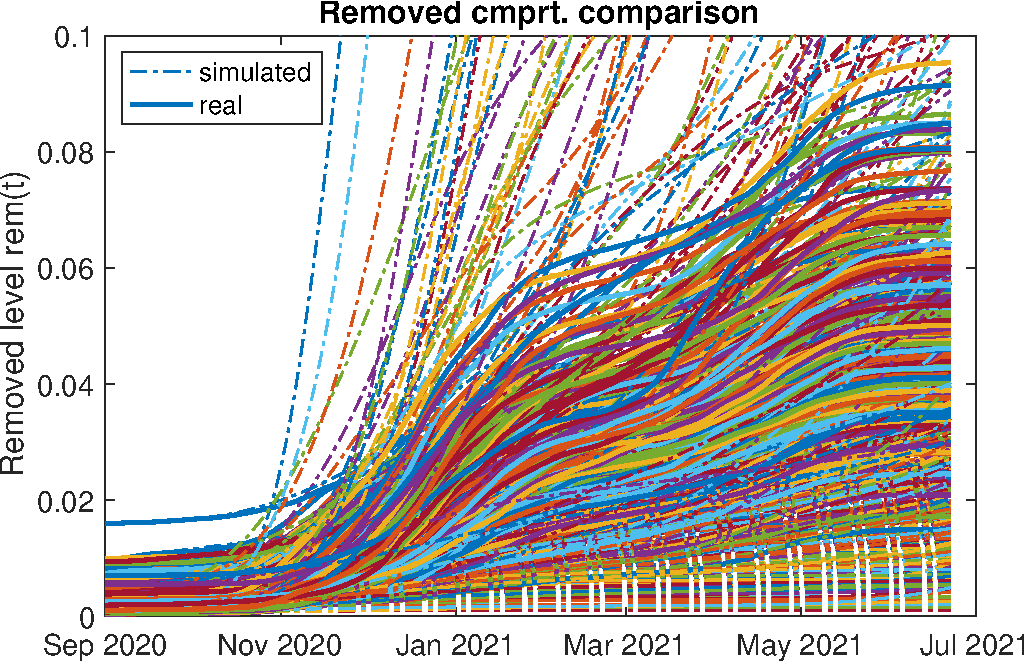
\includegraphics[width=\linewidth]{img/210907_224622_combined_wave23/figures/SEIR_r_sim-vs-real}
         \caption{Removed}
         \label{fig:compCombWave23Rem}
     \end{subfigure}     
     \caption{Compartment levels, waves 2\&3 with combined mobility; left: normalized per county, right: aggregated denormalized}
     \label{fig:compCombWave23}
\end{figure}

\section{Data sets and formats}
This section introduces specialties and caveats about the data sets used in the report and how their specific formats work. The interested reader is guided to other resources for further reading. The data sets are aggregated and made available in their raw form in the following public git repository free of charge using the git LFS technology: \url{https://github.com/hashkode/covid-data}

\subsection{Mobility data - GTFS}
The mobility data used herein is provided by the DELFI e.V. and licensed under \href{https://creativecommons.org/licenses/by/4.0/deed.de}{CC BY 4.0}.\cite{delfie.v.OpenDataOPNV2021}
The data set is provided in the format of GTFS, which is a standardized format originating from Google. The reference documentation for the format describing all involved files, keys and possible uses can be found here: \href{https://developers.google.com/transit/gtfs/reference}{GTFS Reference}.

\subsection{COVID-19 data - RKI}
The COVID-19 data used in this project is taken from the Robert Koch-Institut (RKI). It consists of:
\begin{itemize}
	\item Daily caseload per age group, gender and county for Germany in the form of a timetable \cite{robertkoch-institutrkiRKICOVID192021} licensed under \href{https://www.govdata.de/dl-de/by-2-0}{DL-DE/BY-2.0} and
	\item daily vaccination information on a national and state level \cite{robertkoch-institutrkiRKICoronavirusSARSCoV22021} also licensed under \href{https://www.govdata.de/dl-de/by-2-0}{DL-DE/BY-2.0}.
\end{itemize}

\subsection{Mobility behavior data - DESTATIS}
The mobility data that is used to prepare the behavior vector mentioned in \eqref{eq:6a}, \eqref{eq:6b} and \eqref{eq:6c} is provided by the German Statistics Office named DESTATIS. Two different data sets are used herein:
\begin{itemize}
	\item Relative change in total mobility behavior compared to 2019 levels per county as a timetable \cite{statistischesbundesamtdestatisVeranderungsrateMobilitatGgu2021} licensed for free use with reference \href{https://www.destatis.de/DE/Service/Impressum/copyright-allgemein.html}{DESTATIS - Copyright allgemein} and
	\item Relative change mobility behavior for different modes of travel compared to 2019 levels aggregated on the national level as a timetable \cite{statistischesbundesamtdestatisVerkehrsmittelImFernverkehr2021} licensed for free use with reference \href{https://www.destatis.de/DE/Service/Impressum/copyright-allgemein.html}{DESTATIS - Copyright allgemein}.
\end{itemize}


%%%%%%%%%%%%%%%%%%%%%%%%% References %%%%%%%%%%%%%%%%%%%%%%%%%%%%%%%%%
\bibliography{refs/literature}
\bibliographystyle{ieeetr}


%%%%%%%%%%%%%%%%%%%%%%%%% List of Abrevations %%%%%%%%%%%%%%%%%%%%%%%%%%%%%%%%%
\ifdefined\AddMyGloss
\glsaddall
	\AddMyGloss 
\fi
\end{document}
